\documentclass[12pt]{article}
\raggedbottom
% ==================================================
% CONFIGURACIÓN DE PÁGINA
% ==================================================
\usepackage[
a4paper,
top=3cm,
bottom=3cm,
left=2cm,
right=2cm,
includefoot,
footskip=50pt
]{geometry}

% ==================================================
% IDIOMA Y CODIFICACIÓN
% ==================================================
\usepackage[T1]{fontenc}
\usepackage[utf8]{inputenc}
\usepackage[spanish, es-tabla]{babel}

% ==================================================
% MATEMÁTICAS
% ==================================================
\usepackage{amsmath,amssymb,amsfonts}

% ==================================================
% IMÁGENES Y TABLAS
% ==================================================
\usepackage{graphicx}
\usepackage{tabularx}
\usepackage{array}
\usepackage{booktabs}
\usepackage{float}
\usepackage{caption}
\usepackage{subcaption}

\newcolumntype{Y}{>{\centering\arraybackslash}X}

% ==================================================
% FORMATO DE TEXTO
% ==================================================
\usepackage{titlesec}

\setlength{\parskip}{0.5em}
\setlength{\textfloatsep}{5pt}
\setlength{\intextsep}{10pt}

\parindent=0cm

% Numeración y profundidad
\setcounter{secnumdepth}{5}
\setcounter{tocdepth}{5}

% Formato de párrafos
\titleformat{\paragraph}[block]
{\normalfont\normalsize\bfseries}
{\theparagraph}
{1em}
{}

\titlespacing*{\paragraph}
{0pt}
{1ex plus 0.5ex minus .2ex}
{1ex}

% ==================================================
% ENCABEZADOS Y PIE DE PÁGINA
% ==================================================
\usepackage{fancyhdr}

% ==================================================
% HIPERVÍNCULOS
% ==================================================
\usepackage[
unicode,
colorlinks=true,
linkcolor=black,
urlcolor=blue,
citecolor=black
]{hyperref}

% ==================================================
% BIBLIOGRAFÍA
% ==================================================
\usepackage{csquotes}

\usepackage[
backend=biber,
style=apa,
sortcites,
url=true
]{biblatex}

\addbibresource{biblio.bib}

% ==================================================
% NOMBRES EN ESPAÑOL
% ==================================================
\addto\captionsspanish{
	\renewcommand{\contentsname}{Tabla de contenido}
	\renewcommand{\listfigurename}{Lista de figuras}
	\renewcommand{\listtablename}{Lista de tablas}
}

% ==================================================
% DOCUMENTO
% ==================================================

% ===== DOCUMENTO =====
\begin{document}
	
	
	\begin{titlepage}
		\centering
		
\includegraphics[width=0.2\textwidth]{../figuras/Logo_1.png}\par\vspace{1cm}
		
		
		% Título del trabajo
            {\Huge \textbf{ESTUDIO DE AMENAZA SÍSMICA PARA LA CIUDAD DE NEIVA}}\par
      	\vspace{2.5cm}
		
		% Autores
		{\Large \textbf{ELABORADO POR:}\\
			ANDRÉS STIVEN JARAMILLO CATAÑO\\
			EMMEL ESCOVITHCH RIAÑO\\
                  LAURY YOCELY PEREA MENA\par}
		\vspace{2.5cm}
		
		% Autores
		{\Large \textbf{DOCENTE:}\\
			ANDRES FELIPE SERNA VAZQUEZ\par}
		\vspace{2.5cm}
		
		% Facultad y departamento
		{\large \textbf{
				Universidad Nacional de Colombia\\
				Facultad de Ingeniería\\
				Departamento de Ingeniería Civil}}
		
		\vfill
		% Fecha
		\textbf{{\large OCTUBRE 2026}}
	\end{titlepage}



	
	\pagestyle{fancy}
	
	% Limpiar encabezado y pie
	\fancyhf{}
	
	% ===== ENCABEZADO =====
	\fancyhf{} % limpia todo
	
	\fancyhead[L]{\raisebox{5pt}{
\includegraphics[height=2cm]{../figuras/Logo_encabezado.png}}}
	
	\fancyhead[R]{%
		\raisebox{5pt}{
			\parbox{4cm}{\centering
				\small\textbf{Ingeniería Sismo-Geotécnia}}
		}
	}
	
	
	
	% ===== PIE DE PÁGINA =====
	\fancyfoot[C]{Página \thepage}
	
	% Líneas superior e inferior
	\renewcommand{\headrulewidth}{0.4pt}
      \renewcommand{\footrulewidth}{0pt}

      \fancypagestyle{plain}{%
            \fancyhf{}
            \fancyfoot[C]{\small Página \thepage}
            \renewcommand{\headrulewidth}{0pt}
            \renewcommand{\footrulewidth}{0pt}
      }
	
	% Ajusta la altura del encabezado
      \setlength{\headheight}{66.3pt}
	
	\setlength{\headsep}{30pt}      
	
	
	
\tableofcontents
\listoffigures
	

\newpage

% ============================================================
\section{Introducción}

Este informe documenta el avance del trabajo de amenaza sísmica para la ciudad de
Neiva (Huila). El objetivo del trabajo es construir un catálogo sísmico depurado
para Neiva, a partir de las fuentes del Servicio Geológico Colombiano (SGC) y del
United States Geological Survey (USGS), dentro de radios de 50~km y 260~km medidos
desde un punto de referencia en el centro de la ciudad. Este catálogo es el insumo
principal para el posterior análisis de amenaza sísmica, la construcción del
espectro en roca según la NSR-10 y la selección de acelerogramas compatibles.

Este documento recoge las etapas de recopilación, homogenización de magnitudes,
depuración espacio-temporal y análisis frecuencia--magnitud, además de dejar
señalados los pasos pendientes para el análisis de amenaza sísmica.

% ============================================================
\section{Objetivos}

\begin{itemize}
    \item Construir un catálogo sísmico homogenizado en magnitud de momento
          $M_w$ para la ciudad de Neiva y sus radios de estudio.
    \item Aplicar y comparar cuatro criterios de depuración de réplicas y
          precursores sobre una población común con $M_w>3.0$.
    \item Estimar la distribución frecuencia--magnitud y los parámetros
          exploratorios de Gutenberg--Richter para cada método.
    \item Dejar preparada la base para asociar los eventos depurados con las
          sismofuentes regionales en una etapa posterior.
\end{itemize}

% ============================================================
\section{Descripción del proyecto}

Como punto de referencia para la búsqueda del catálogo sísmico se adoptó el
\textbf{Parque Central Santander}, en el centro cívico e institucional de Neiva,
con coordenadas:

\begin{center}
    Latitud: $2.9262767$\textdegree \qquad Longitud: $-75.2892111$\textdegree
\end{center}

A partir de este punto se definieron dos radios de búsqueda:

\begin{itemize}
    \item \textbf{50 km}: catálogo cercano, relevante para la amenaza sísmica
          local y la sismicidad asociada a fuentes próximas a la ciudad.
    \item \textbf{260 km}: catálogo regional, que permite capturar fuentes
          sismogénicas distantes (por ejemplo, la subducción del Pacífico y
          sistemas de falla regionales) que también pueden contribuir a la
          amenaza sísmica de Neiva. Este radio se adoptó, en lugar de uno de
          200~km, para garantizar que la sismicidad asociada al municipio de
          San José del Palmar (Chocó) quede dentro de la zona de estudio: sus
          epicentros se encuentran entre 232 y 260~km del punto de referencia.
    \end{itemize}

La Figura~\ref{fig:mapa_zona} muestra el punto de referencia y ambos radios
de búsqueda sobre una imagen satelital de la región. Neiva se encuentra en
el valle interandino del Alto Magdalena, entre las cordilleras Central y
Oriental; el radio de 260~km alcanza ciudades como Cali, Ibagué, Popayán y
Bogotá, y se extiende hasta la zona de subducción del Pacífico.

\begin{figure}[H]
    \centering
    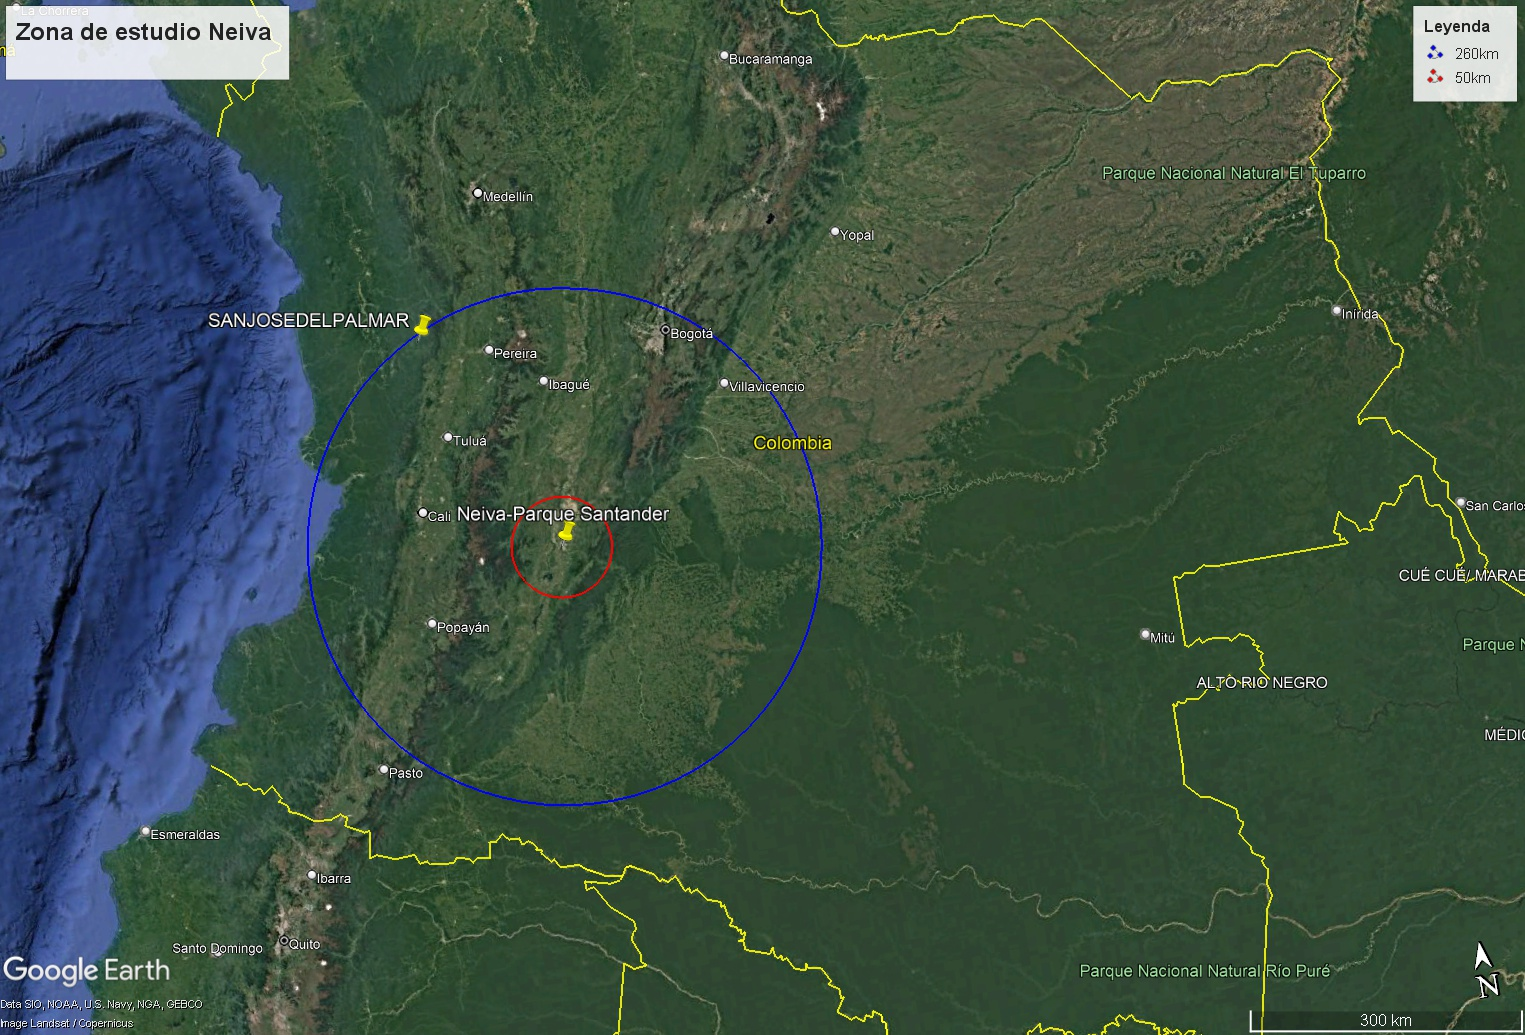
\includegraphics[width=0.8\textwidth]{../figuras/zonadeestudioradio260.jpg}
    \caption{Zona de estudio: punto de referencia en Neiva (Parque Central
    Santander), radios de búsqueda de 50 y 260~km y ubicación de San José del
    Palmar. Imagen satelital: Google Earth.}
    \label{fig:mapa_zona}
\end{figure}

Como primer acercamiento a la sismicidad de la zona, la Figura~\ref{fig:mapa_epicentros}
muestra los epicentros del catálogo consolidado (SGC y USGS) dentro de
260~km, coloreados por magnitud y diferenciados por fuente (círculos para
el SGC, triángulos para el USGS). Se aprecia una alineación de sismicidad
de suroeste a noreste, consistente con el sistema de fallas regional de la
zona (Algeciras--Suaza), además de un cúmulo de sismicidad más profunda
hacia el occidente, asociado a la zona de subducción. Los eventos del USGS
se concentran en las magnitudes más altas de cada zona, consistente con lo
discutido en la Sección~\ref{sec:estado}.

\begin{figure}[H]
    \centering
    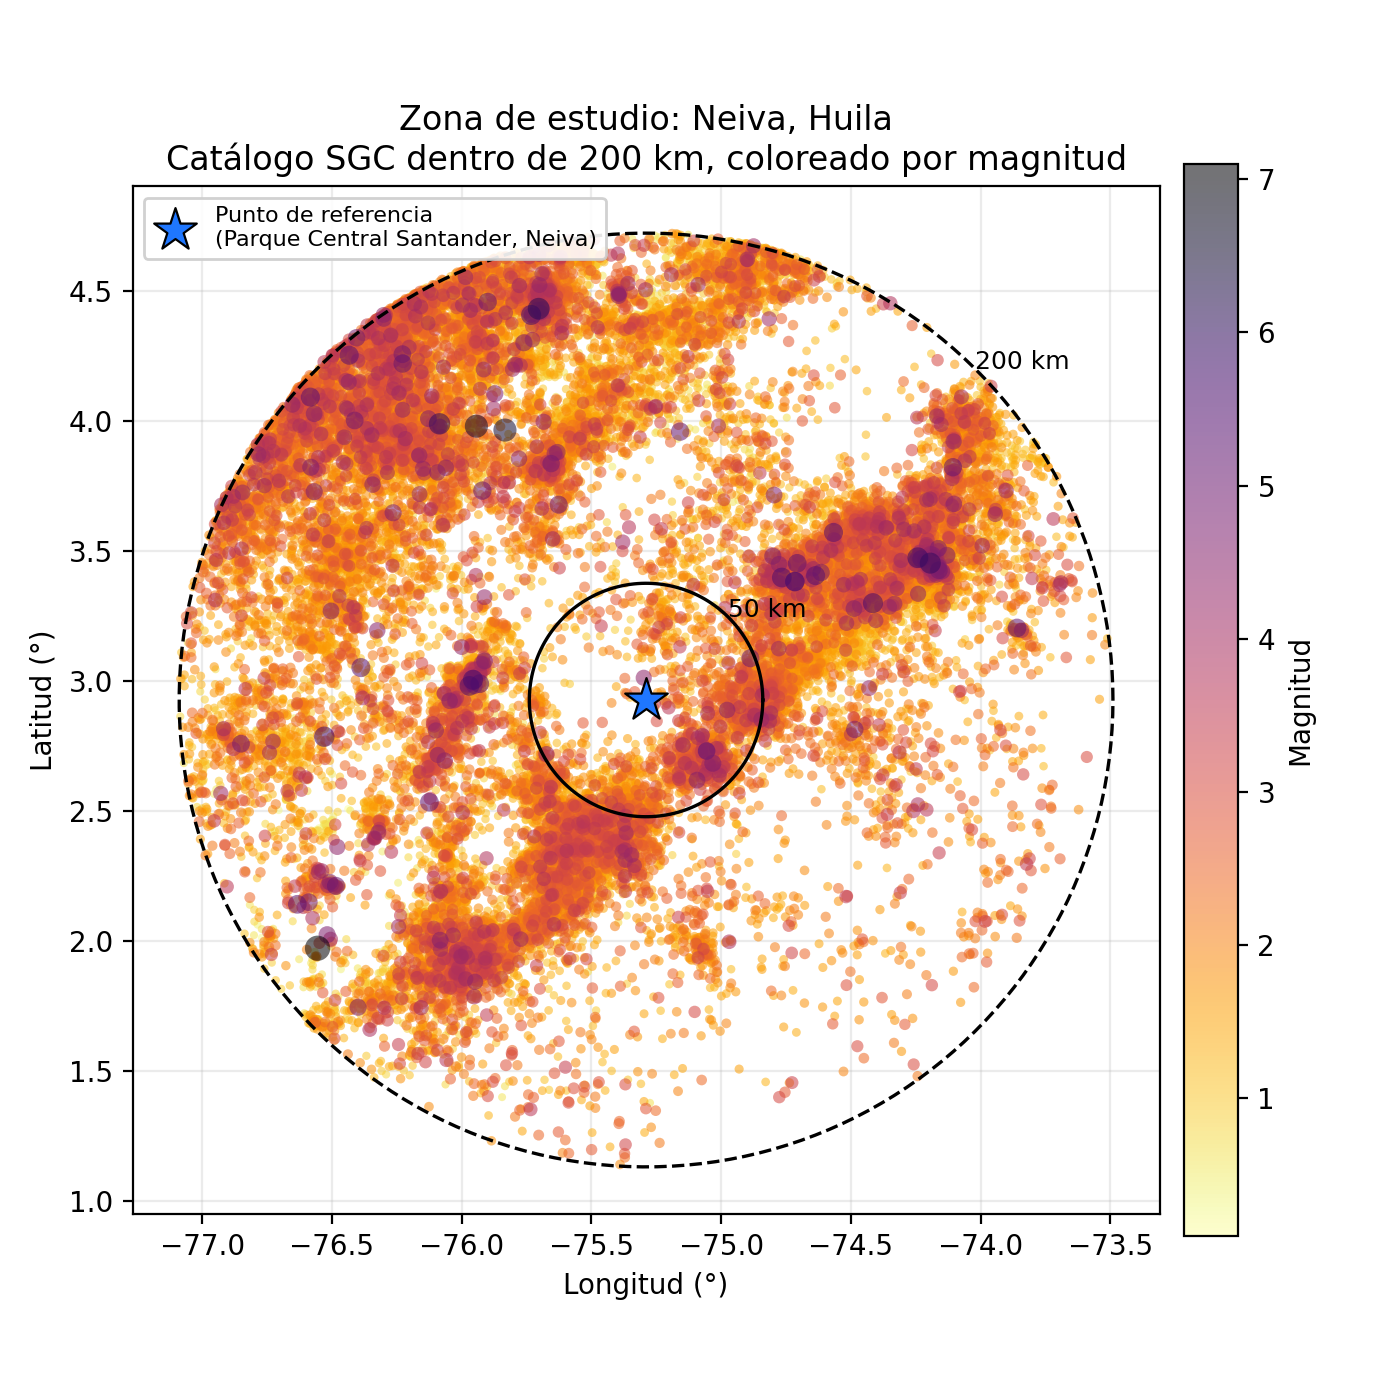
\includegraphics[width=0.85\textwidth]{../figuras/mapa_zona_estudio.png}
    \caption{Epicentros del catálogo consolidado SGC + USGS dentro de
    260~km alrededor de Neiva, coloreados por magnitud y diferenciados por
    fuente.}
    \label{fig:mapa_epicentros}
\end{figure}

% ============================================================
\subsection{Fuentes de datos utilizadas}

Se utilizaron dos fuentes de información sismológica:

\begin{itemize}
    \item \textbf{SGC -- Red Sismológica Nacional de Colombia (RSNC)}: catálogo
          oficial de sismicidad de Colombia, operado por el Servicio Geológico
          Colombiano. Por ser una red local densa, este catálogo captura
          microsismicidad (magnitudes menores a 2) que las redes globales no
          alcanzan a detectar cerca del territorio colombiano
          \parencite{sgcCatalogoSismicidad}.
    \item \textbf{USGS -- ANSS Comprehensive Earthquake Catalog (ComCat)}:
          catálogo global del United States Geological Survey, construido a
          partir de redes sismológicas mundiales. Es comparativamente completo
          para sismos grandes (magnitud $\gtrsim 4$), pero no detecta de forma
          confiable la microsismicidad local \parencite{usgsComCat}.
\end{itemize}

\subsection{Parámetros de búsqueda}

Para las cuatro combinaciones de fuente y radio se utilizó el mismo punto de
referencia, sin límite inferior de magnitud (magnitud mínima $=0$, es decir,
sin filtrar) y considerando el rango histórico completo disponible en cada
fuente, con el fin de conservar el catálogo lo más completo posible. Los
parámetros específicos se resumen en el Cuadro~\ref{tab:parametros}.

\begin{table}[H]
    \centering
    \caption{Parámetros de búsqueda utilizados por fuente.}
    \label{tab:parametros}
    \begin{tabular}{lll}
        \toprule
        Parámetro & SGC & USGS \\
        \midrule
        Servicio / endpoint & \texttt{apicatalogador.sgc.gov.co} & \texttt{earthquake.usgs.gov} (FDSN) \\
        Centro de búsqueda & lat/lon del punto de referencia & lat/lon del punto de referencia \\
        Radios & 50 km y 260 km & 50 km y 260 km \\
        Magnitud mínima & sin filtro (0) & 0 \\
        Rango de fechas & histórico completo & 1900-01-01 -- fecha de descarga \\
        Formato de salida & JSON $\rightarrow$ CSV & CSV \\
        \bottomrule
    \end{tabular}
\end{table}

\subsection{Decisiones metodológicas}

Durante la recopilación del catálogo se tomaron las siguientes decisiones,
que se documentan aquí por su relevancia para la trazabilidad del trabajo:

\begin{itemize}
    \item \textbf{Elección del punto de referencia.} Se adoptó el Parque
          Central Santander por ser el centro cívico e institucional de Neiva,
          un punto estable y fácilmente verificable en cartografía, en lugar
          de, por ejemplo, el centroide del área urbana o la ubicación de una
          estación acelerográfica particular.

    \item \textbf{Catálogo completo del SGC, no solo el resultado por defecto
          de la interfaz web.} La herramienta de consulta pública del SGC
          (\url{https://sismo.sgc.gov.co}) internamente restringe o pagina los
          resultados que muestra en pantalla. Se identificó el servicio REST
          que alimenta la página oficial de descarga del catálogo
          (\texttt{https://apicatalogador.sgc.gov.co/api/events/search/}), y se
          consultó de forma paginada (1000 registros por página) hasta reunir
          la totalidad de los eventos reportados dentro de cada radio, en
          lugar de conformarse con un subconjunto parcial
          \parencite{sgcApiEventos}.

    \item \textbf{Sin filtro de magnitud mínima.} Siguiendo la regla de
          trabajo acordada de no descartar información sin autorización
          explícita, se dejó la magnitud mínima en 0 en ambas fuentes, de
          modo que el catálogo conserve incluso los sismos de magnitud muy
          baja. La depuración de réplicas se realiza después, sin aplicar un
          umbral artificial de magnitud.

    \item \textbf{Corrección de codificación de caracteres.} En la descarga
          automatizada del catálogo del SGC se detectó y corrigió un problema
          de codificación que producía caracteres corruptos en los nombres de
          municipios con tildes o eñes (por ejemplo, ``Caguán'' o
          ``Caquetá''), asegurando que el texto se decodificara correctamente
          como UTF-8.

    \item \textbf{Dos fuentes, no una sola.} Se mantienen ambos catálogos
          (SGC y USGS) por separado en \texttt{datos originales/} en lugar de
          usar solo uno, dado que son complementarios: el SGC aporta
          completitud en magnitudes bajas y el USGS aporta soluciones
          independientes (incluyendo magnitud de momento $M_w$) útiles para
          la homogenización de escalas de magnitud en la siguiente etapa.

    \item \textbf{Fila duplicada por la descarga.} En el catálogo del SGC a
          260~km, el evento SGC2015gaurko apareció dos veces con datos
          idénticos por un solapamiento entre páginas de la descarga; se
          conservó una sola copia. No se eliminó ningún otro registro.
\end{itemize}

% ============================================================
\subsection{Estado actual del catálogo}
\label{sec:estado}

El Cuadro~\ref{tab:estado} resume el estado inicial de los cuatro catálogos
considerados en el análisis.

\begin{table}[H]
    \centering
    \caption{Estado actual de los catálogos descargados.}
    \label{tab:estado}
    \begin{tabular}{llrrr}
        \toprule
        Fuente & Radio & N.\ de eventos & Magnitud mín. & Magnitud máx. \\
        \midrule
        SGC  & 50 km  & 2\,380  & 0.7    & 5.0 \\
        SGC  & 260 km & 67\,781 & $-0.1$ & 7.4 \\
        USGS & 50 km  & 20      & 3.4    & 5.5 \\
        USGS & 260 km & 823     & 0.0    & 7.4 \\
        \bottomrule
    \end{tabular}
\end{table}

Se observa una diferencia de casi dos órdenes de magnitud entre el número de
eventos del SGC y del USGS para el mismo radio. Esto es un resultado esperado
y no un error: el SGC opera una red local densa que detecta sismicidad de
magnitud muy baja cerca del territorio colombiano, mientras que el catálogo
global del USGS solo es razonablemente completo para magnitudes mayores a,
aproximadamente, 3.5--4.0 en esta región. En el rango de sismos grandes
($M \geq 4$) ambos catálogos reportan cantidades del mismo orden a 260~km (400
eventos en el SGC y 454 en el USGS), lo que es consistente con esta
explicación. Que el USGS reporte algo más se debe, en buena parte, a su
cobertura temporal: su catálogo inicia en 1917, mientras que el del SGC inicia
en 1993 (desde 1993, el USGS reporta 319 eventos con $M \geq 4$).

Los catálogos se descargaron el 21 de septiembre de 2026. Las magnitudes de
cada fuente se presentan en su escala original; aún no se han homogenizado.

% ============================================================
\section{Marco teórico}

\subsection{Homogenización de magnitudes}
\label{sec:conversion_magnitudes}

La homogenización consiste en expresar, en una escala común, magnitudes que
fueron calculadas a partir de amplitudes, períodos o duraciones diferentes.
Para este trabajo se adopta la magnitud de momento sísmico $M_w$ como escala
de referencia. Esta elección es apropiada porque $M_w$ está relacionada con el
momento sísmico de la fuente y, a diferencia de las magnitudes basadas en
amplitud, conserva una relación más estable con el tamaño de los terremotos
grandes. Sin embargo, una magnitud convertida no es una observación directa de
$M_w$: es un estimador empírico, por lo que debe conservarse su ecuación,
rango de validez y dispersión.

\subsection{Definición de las escalas}

El momento sísmico escalar se define como
\begin{equation}
      M_0 = \mu A D,
      \label{eq:momento_sismico}
\end{equation}
donde $\mu$ es el módulo de rigidez, $A$ es el área de ruptura y $D$ es el
deslizamiento medio. La relación convencional entre $M_0$, expresado en
N\,m, y la magnitud de momento es
\begin{equation}
      M_w = \frac{2}{3}\left(\log_{10} M_0 - 9.1\right).
      \label{eq:mw_momento}
\end{equation}
Las constantes de la ecuación dependen del sistema de unidades; por ello no se
debe combinar esta expresión con un $M_0$ expresado en dyn\,cm sin modificar la
constante.

Las escalas que pueden aparecer en los catálogos consultados tienen distinto
significado: $M_L$ es magnitud local, $M_d$ o $M_c$ es magnitud de duración o
coda, $m_b$ es magnitud de ondas de cuerpo de período corto, $M_s$ es magnitud
de ondas superficiales, $M_{SK}$ es una variante regional de ondas
superficiales y $M_{JMA}$ es la escala de la Agencia Meteorológica de Japón.
También pueden aparecer $m_B$ y magnitudes locales regionales como $M_{Lr}$.
Los símbolos parecidos no deben tratarse como equivalentes: por ejemplo,
$m_b$ y $m_B$ utilizan bandas de período diferentes y requieren calibraciones
distintas.

\subsection{Forma general de las relaciones empíricas}

La forma más común es una regresión lineal
\begin{equation}
      \widehat{M_w}=a+bX,
      \label{eq:lineal_conversion}
\end{equation}
donde $X$ es la magnitud observada. Cuando la relación cambia por saturación o
por transición entre regímenes, se utiliza una función bilineal o por tramos,
\begin{equation}
      \widehat{M_w}=\begin{cases}
      a_1+b_1X, & X\leq X_c,\\
      a_2+b_2X, & X>X_c.
      \end{cases}
      \label{eq:bilineal_conversion}
\end{equation}
La continuidad en $X_c$ no debe suponerse si los autores no la impusieron en el
ajuste. Lolli, Gasperini y Vannucci también evaluaron modelos curvilíneos; su
forma exponencial recomendada, con $\exp$ la exponencial natural, es
\begin{equation}
      \widehat{M_w}=\exp(a+bX)+c.
      \label{eq:exponencial_conversion}
\end{equation}
Estos modelos son preferibles cuando la pendiente cambia progresivamente y no
en un único punto de quiebre \parencite{lolli2014empirical}.

\subsection{Relaciones globales verificadas}

\subsubsection{Relaciones de Scordilis y Bormann--Saul}

Las relaciones globales de Scordilis, reproducidas por Bormann y Saul, fueron
ajustadas con grandes catálogos internacionales. Para $M_s$ se obtienen dos
tramos:
\begin{align}
      M_w &= 0.65M_s+2.20, &&3.0\leq M_s\leq6.1, &&\sigma=0.17,\\
      M_w &= 1.00M_s-0.02, &&6.2\leq M_s\leq8.0, &&\sigma=0.21.
      \label{eq:scordilis_ms}
\end{align}
Para $M_{SK}$, considerado equivalente a $M_s$ en el ámbito regional de esa
fuente, se reportan tres tramos:
\begin{align}
      M_w &= 0.78M_{SK}+1.45, &&4.0\leq M_{SK}\leq5.3, &&\sigma=0.42,\\
      M_w &= 0.68M_{SK}+1.99, &&5.4\leq M_{SK}\leq6.1, &&\sigma=0.32,\\
      M_w &= 1.04M_{SK}-0.30, &&M_{SK}\geq6.2, &&\sigma=0.34.
      \label{eq:scordilis_msk}
\end{align}
Para la magnitud de ondas de cuerpo y la escala JMA se obtienen:
\begin{align}
      M_w &= 0.85m_b+1.02, &&3.5\leq m_b\leq6.2, &&\sigma=0.29,\\
      M_w &= 0.58M_{JMA}+2.25, &&3.0\leq M_{JMA}\leq5.5, &&\sigma=0.28,\\
      M_w &= 0.97M_{JMA}+0.04, &&5.6\leq M_{JMA}\leq8.2, &&\sigma=0.22.
      \label{eq:scordilis_mb_jma}
\end{align}
Estas ecuaciones son globales y no sustituyen una calibración local. Además,
$m_b$ presenta saturación aproximada para valores superiores a 6.2--6.3, razón
por la cual no debe extrapolarse la primera expresión a terremotos grandes
\parencite{bormann2005globally}.

\subsubsection{Relaciones de Lolli, Gasperini y Vannucci}

Lolli et al. compararon regresión ortogonal generalizada y regresión no lineal
para magnitudes teleseísmicas. Sus recomendaciones finales para un uso global
son, para $M_s$:
\begin{equation}
 \widehat{M_w}=\begin{cases}
 \exp(2.133+0.063M_s)-6.205, & M_s\leq5.5,\\
 \exp(-0.109+0.229M_s)+2.586, & M_s>5.5,
 \end{cases}
 \label{eq:lolli_ms_global}
\end{equation}
y para $m_b$:
\begin{equation}
      \widehat{M_w}=\exp(0.741+0.210m_b)-0.785.
      \label{eq:lolli_mb_global}
\end{equation}
Para comparación, el estudio reporta las siguientes expresiones alternativas:
\begin{align}
      \widehat{M_w}&=\exp(2.133+0.063M_s)-6.205 &&\text{(Euro-Mediterráneo)},\\
      \widehat{M_w}&=\exp(0.719+0.212m_b)-0.737 &&\text{(Euro-Mediterráneo)},\\
      \widehat{M_w}&=\exp(1.421+0.108M_s)-1.863 &&\text{(Italia)},\\
      \widehat{M_w}&=\exp(0.058+0.284m_b)-0.770 &&\text{(Italia)}.
      \label{eq:lolli_regionales}
\end{align}
Para valores globales de $M_s\leq5.5$, los autores recomiendan la relación
Euro-Mediterránea debido a la subrepresentación de terremotos pequeños en los
catálogos globales de tensor de momento. Esta observación es relevante para el
catálogo de Neiva: una fórmula ajustada con eventos grandes no debe aplicarse
automáticamente a la abundante microsismicidad del SGC
\parencite{lolli2014empirical}.

\subsection{Relaciones para magnitudes locales y de duración}

Senel et al. ajustaron relaciones para Turquía usando regresión ortogonal para
$M_s$ y mínimos cuadrados ordinarios para $m_b$, $M_L$ y $M_d$. Las ecuaciones
propuestas son:
\begin{align}
      M_w &= 0.5716M_s+2.4980, &&3.4\leq M_s\leq5.4,\\
      M_w &= 0.8126M_s+1.1723, &&M_s\geq5.5,\\
      M_w &= 1.0319m_b+0.0223, &&3.9\leq m_b\leq6.8,\\
      M_w &= 0.8095M_L+1.3003, &&3.3\leq M_L\leq6.6,\\
      M_w &= 0.7947M_d+1.3420, &&3.5\leq M_d\leq7.4.
      \label{eq:senel}
\end{align}
La cuarta expresión se escribe con $M_L$ porque así se reporta en el artículo;
la quinta usa $M_d$. El rango original, el método de ajuste y la región de
calibración deben acompañar siempre a cada valor convertido
\parencite{senel2016new}.

\subsection{Relaciones regionales y límites de transferencia}

Tang, Zhu y Huang encontraron calibraciones específicas para China occidental
entre $M_w$ y $M_L$, $m_b$ y $M_s$, usando regresión ortogonal generalizada.
El artículo muestra que las pendientes y dispersión cambian entre las tres
zonas tectónicas estudiadas y que las relaciones globales de Lolli presentan
dispersión mayor para ese conjunto. Por tanto, sus ecuaciones regionales no se
transfieren numéricamente a Colombia; sí son evidencia de que el entorno
tectónico debe considerarse al escoger una relación
\parencite{tang2016empirical}.

Para Cuba, Jamaica y La Española, Villalón-Semanat y Palau-Clares ajustaron
relaciones entre $m_b$, $M_s$, $M_w$ y $M_c$. El estudio confirma una buena
correlación $M_s$--$M_w$ en el rango aproximado $3.8$--$7.0$, pero advierte
que la relación $m_b$--$M_c$ tiene gran dispersión y no debe utilizarse para
homogenizar catálogos. Esto es especialmente importante para nuestro caso:
una magnitud de coda o duración del SGC no se convertirá mediante una cadena
de fórmulas sucesivas sin una calibración colombiana independiente
\parencite{villalon2018relaciones}.

\subsection{Criterio de selección para el catálogo de Neiva}

El procedimiento propuesto para cada registro es el siguiente:
\begin{enumerate}
      \item Conservar la magnitud original, su tipo, agencia y fecha de cálculo;
      \item usar el $M_w$ observado por USGS o por otra solución de tensor de
      momento cuando exista, sin reemplazarlo por una conversión;
      \item para $m_b$ o $M_s$, usar inicialmente una relación global dentro de
      su rango publicado y registrar la ecuación elegida;
            \item para $M_L$, $M_{Lr}$ y $M_{MLr}$, aplicar como estimador
            provisional la relación de Senel et al. y marcar como extrapolados los
            valores fuera de $3.3\leq M_L\leq6.6$; para $M_d$ usar su relación
            específica, dentro de $3.5\leq M_d\leq7.4$;
      \item si un evento tiene varias magnitudes convertibles, calcular cada
      estimador por separado y conservar la dispersión entre estimadores, en vez
      de promediarlos sin ponderación;
      \item marcar como extrapolación cualquier valor fuera del rango de ajuste,
      y no convertir magnitudes desconocidas, negativas o con banderas de baja
      calidad sin una revisión adicional.
\end{enumerate}

No debe encadenarse, por ejemplo, $M_L\rightarrow m_b\rightarrow M_w$:
cada conversión añade error y puede propagar el sesgo de saturación. En la
implementación del catálogo, los tipos $M$ y $M_{Pac}$, así como los registros
sin tipo, quedan como \texttt{no\_convertida} porque su definición no es suficiente
para seleccionar una correlación verificable. Las escalas $M_w$, $M_{ww}$,
$M_{wc}$, $M_{wb}$, $M_{wr}$ y $M_{wp}$ se conservan como magnitudes directas.

El catálogo homogenizado conserva la magnitud original y su escala de
determinación, y asocia a cada evento una magnitud $M_w$ directa o estimada,
la relación de conversión utilizada, su incertidumbre y su condición de
validez. Esta última distingue entre magnitudes directas, conversiones dentro
del rango empírico, extrapolaciones y magnitudes no convertidas. Así se evita
confundir un valor convertido fuera del rango publicado con una observación
directa de $M_w$.

\subsection{Incertidumbre de las magnitudes convertidas}

Para una relación lineal $\widehat{M_w}=a+bX$, una aproximación mínima de la
incertidumbre es
\begin{equation}
      \sigma_{\widehat{M_w}}^2 \simeq
      \sigma_{\mathrm{reg}}^2+b^2\sigma_X^2,
      \label{eq:incertidumbre_lineal}
\end{equation}
donde $\sigma_{\mathrm{reg}}$ es la desviación estándar de los residuos y
$\sigma_X$ la incertidumbre de la magnitud de entrada. Si se conocen las
covarianzas de los coeficientes, la forma general es
\begin{equation}
 \sigma_{\widehat{M_w}}^2=\sigma_{\mathrm{reg}}^2+
 \begin{bmatrix}1&X\end{bmatrix}
 \operatorname{Cov}(a,b)
 \begin{bmatrix}1\\X\end{bmatrix}+b^2\sigma_X^2.
 \label{eq:incertidumbre_covarianza}
\end{equation}
Para una relación no lineal $f(X)$, se usa la aproximación de primer orden
$\sigma_{\widehat{M_w}}^2\simeq\sigma_{\mathrm{reg}}^2+[f'(X)]^2\sigma_X^2$.
En consecuencia, el catálogo depurado debe conservar, como mínimo, la
magnitud original, $M_w$ directo o estimado, la relación aplicada, el rango de
validez, la desviación estándar publicada y una bandera de extrapolación. Esta
estructura permite que el análisis de amenaza separe la incertidumbre
aleatoria de la incertidumbre epistemológica asociada a escoger una relación
entre varias.

\section{Desarrollo y análisis}

\subsection{Criterio común de magnitud}
\label{sec:filtro_magnitud_comun}

Antes de aplicar cualquiera de los métodos de depuración se estableció un
catálogo común con eventos que cumplen $M_w>3.0$. Este umbral permite comparar
Gardner--Knopoff, GKL, vecino más cercano y el Criterio propio sobre la misma
población. Los
registros con $M_w\leq3.0$ se conservan en los archivos de exclusiones,
identificados como \texttt{magnitud\_baja}, pero no participan en los
algoritmos de réplicas.

El catálogo elegible contiene 692 eventos para 50 km y 16\,160 eventos para
260 km. Sobre esta misma base se aplican los cuatro criterios descritos a
continuación.

\subsection{Completitud del catálogo}
\label{sec:completitud}

La completitud representa el rango de magnitudes para el cual la red y el
proceso de integración de fuentes registran de manera suficientemente
uniforme los eventos. No debe confundirse con el filtro operativo $M_w>3.0$:
este último define la población de entrada, mientras que $M_c$ se estima a
partir de la distribución de magnitudes del catálogo ya depurado. En este
trabajo se construyó un histograma con intervalos de $0.1$ unidades y se tomó
como estimación exploratoria el centro del intervalo con mayor frecuencia. Por
eso, con bins de $3.0$--$3.1$, el resultado aparece como $M_c=3.05$.

Este valor es una aproximación dependiente del ancho y del origen de los
intervalos; no constituye por sí solo una demostración de completitud física.
La completitud definitiva debe evaluarse por fuente, período, cobertura de la
red y escala de magnitud, además de comprobarse con métodos alternativos. Los
parámetros $b$ y $R^2$ se estiman únicamente para $M_w\geq M_c$.

\subsection{Depuración de réplicas y precursores}
\label{sec:depuracion_replicas}

Antes de construir la distribución frecuencia--magnitud se eliminaron las
réplicas y los precursores mediante el método de ventanas espacio--tiempo de
Gardner y Knopoff \parencite{gardner1974isoseismal}. Los eventos se ordenaron
de mayor a menor $M_w$; para cada evento principal se asignó una ventana
temporal $T(M_w)$ y una distancia máxima $R(M_w)$ mediante interpolación de la
tabla de ventanas. Un evento se marcó como réplica si
ocurrió después del principal, o como precursor si ocurrió antes, siempre que
la diferencia temporal y la distancia epicentral cumplieran ambas condiciones
de la ventana. Los eventos principales se conservaron y cada exclusión quedó
registrada con el identificador y la magnitud del evento que la originó.

La tabla utilizada fue la siguiente. $T$ representa la escala temporal en días
y $R$ la escala espacial en kilómetros:

\begin{table}[H]
      \centering
      \caption{Ventanas espacio--tiempo adoptadas para la depuración Gardner--Knopoff.}
      \label{tab:ventanas_gk}
      \small
      \begin{tabular}{ccc}
            \toprule
            $M_w$ & $T(M_w)$ (días) & $R(M_w)$ (km) \\
            \midrule
            2.0 & 1   & 5   \\
            2.5 & 1   & 5   \\
            3.0 & 2   & 5   \\
            3.5 & 3   & 5   \\
            4.0 & 4   & 10  \\
            4.5 & 6   & 15  \\
            5.0 & 10  & 20  \\
            5.5 & 15  & 30  \\
            6.0 & 22  & 50  \\
            6.5 & 32  & 70  \\
            7.0 & 42  & 90  \\
            7.5 & 83  & 120 \\
            8.0 & 155 & 150 \\
            8.5 & 290 & 180 \\
            9.0 & 510 & 210 \\
            \bottomrule
      \end{tabular}
\end{table}

Para magnitudes entre los valores tabulados se aplicó interpolación lineal.
Para magnitudes menores que $2.0$ o mayores que $9.0$ se utilizaron,
respectivamente, los valores de los extremos de la tabla. La condición de
exclusión fue
\begin{equation}
      |t_i-t_j|\leq T(M_{w,j})
      \quad\text{y}\quad
      d_{ij}\leq R(M_{w,j}),
      \label{eq:criterio_gk}
\end{equation}
donde $j$ es el evento principal, $i$ es el evento candidato y $d_{ij}$ es la
distancia epicentral calculada mediante la fórmula de Haversine. La ventana
temporal se aplicó de forma simétrica, por lo que se identificaron tanto
réplicas posteriores como precursores anteriores. Esta decisión es una
aproximación conservadora del método de ventanas: cuando varios eventos podían
explicar la exclusión, el evento de mayor magnitud procesado primero tuvo
prioridad.

El catálogo elegible de 50~km pasó de 692 a 691 eventos, con una réplica
excluida. El de 260~km pasó de 16\,160 a 16\,012 eventos, con 116 réplicas
y 32 precursores excluidos. Para cada exclusión se conserva la identificación
del evento principal y la magnitud que determinó la ventana aplicada.

\begin{figure}[H]
      \centering
      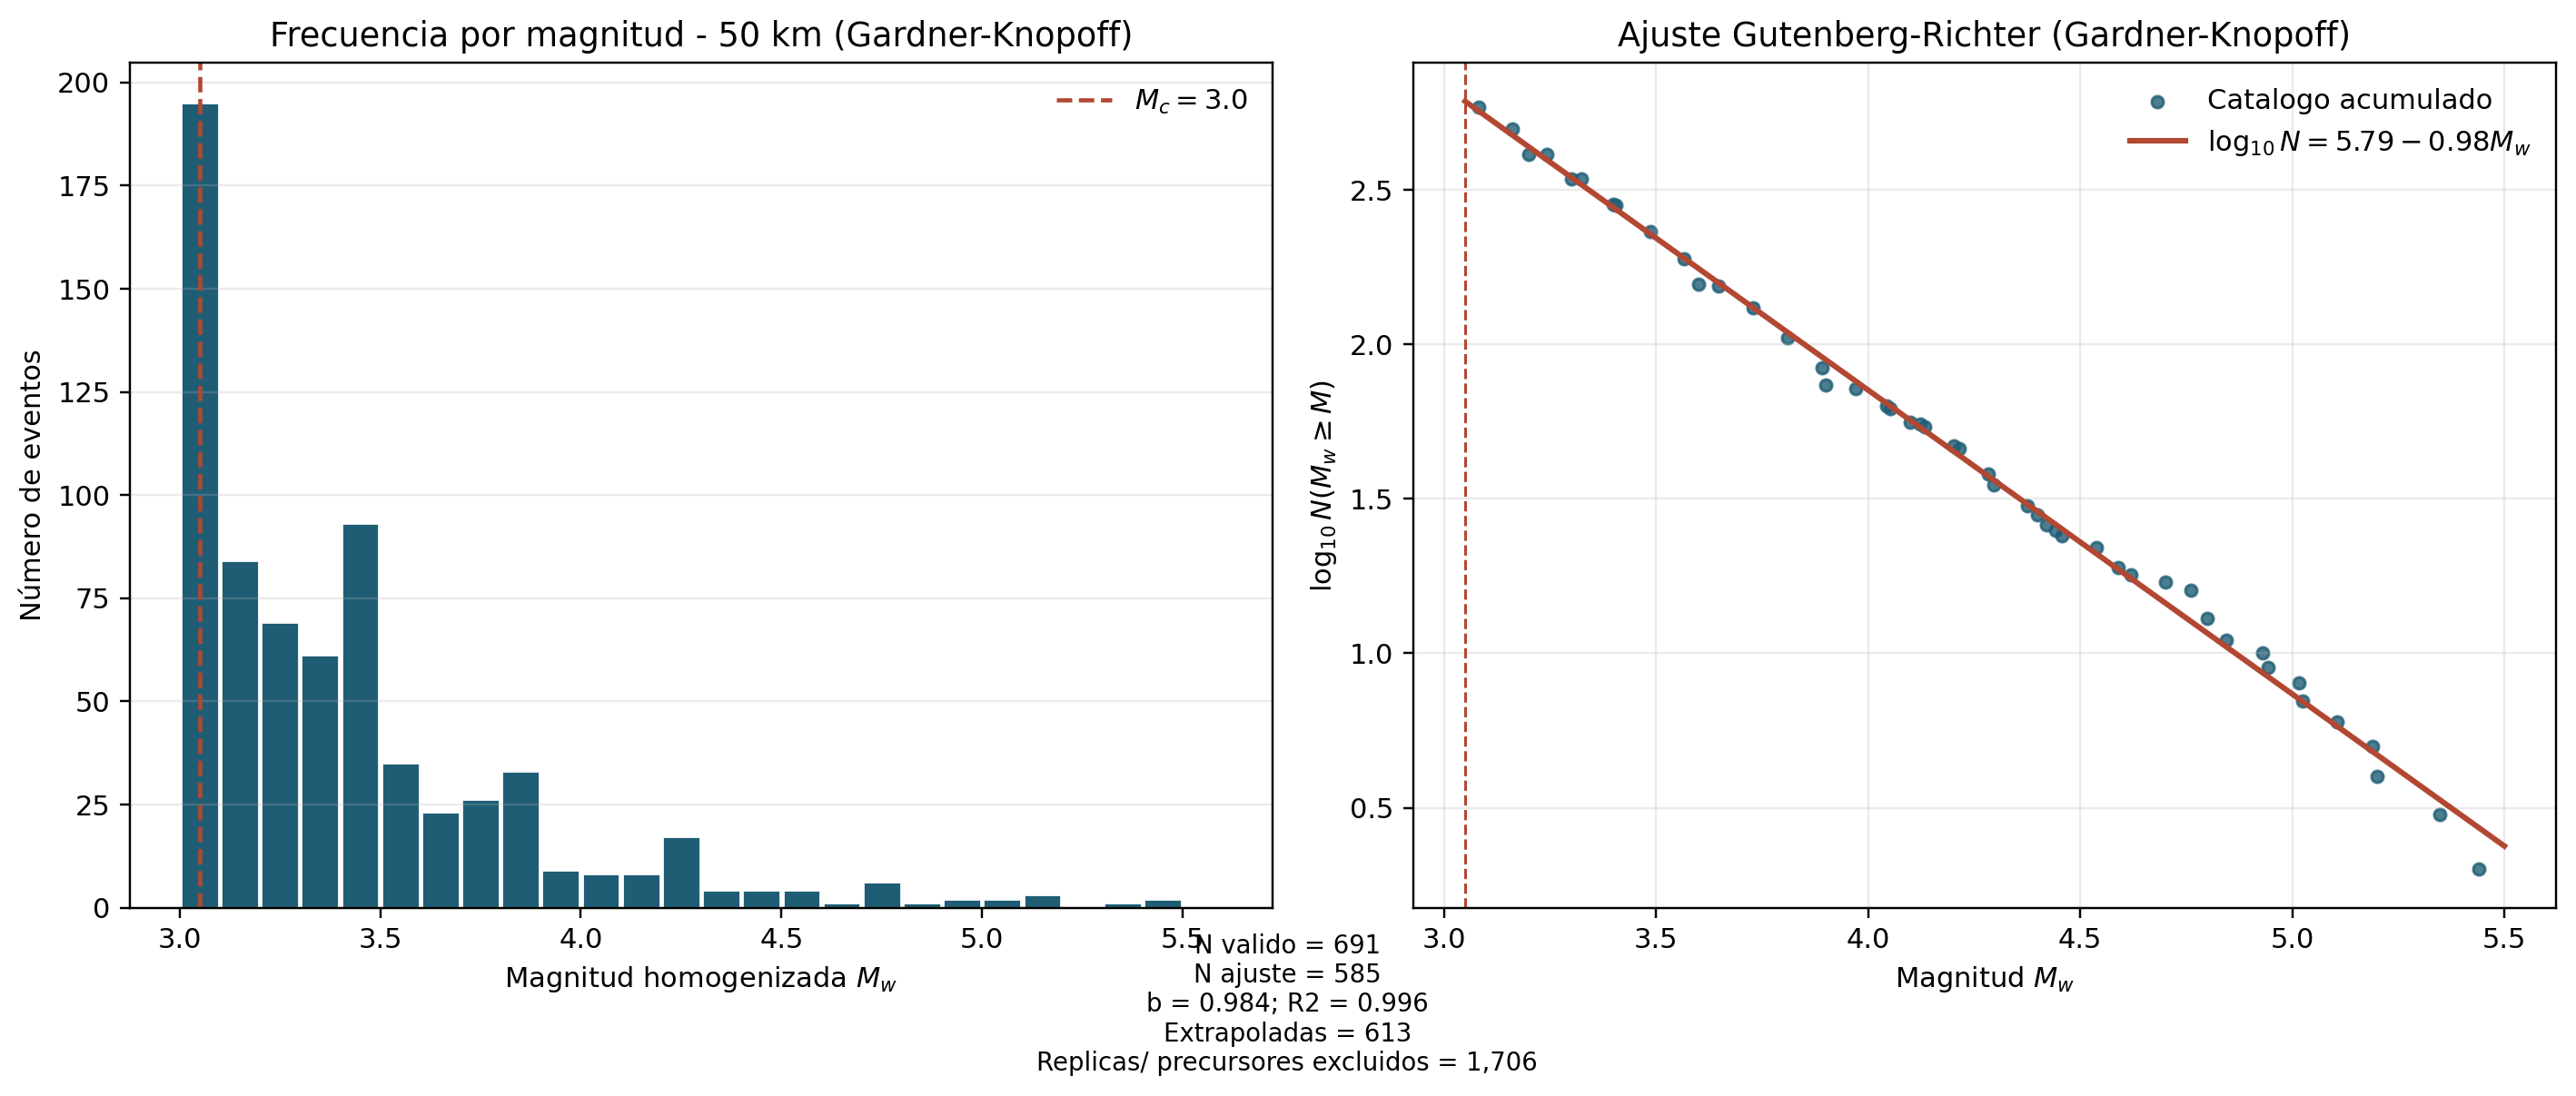
\includegraphics[width=0.92\textwidth]{../figuras/frecuencia_magnitud_50km_gk.png}
      \caption{Frecuencia y ajuste Gutenberg--Richter para el catálogo depurado a 50 km con el método Gardner--Knopoff. La línea vertical indica la magnitud de completitud exploratoria $M_c=3.05$.}
      \label{fig:frecuencia_50km}
\end{figure}

\begin{figure}[H]
      \centering
      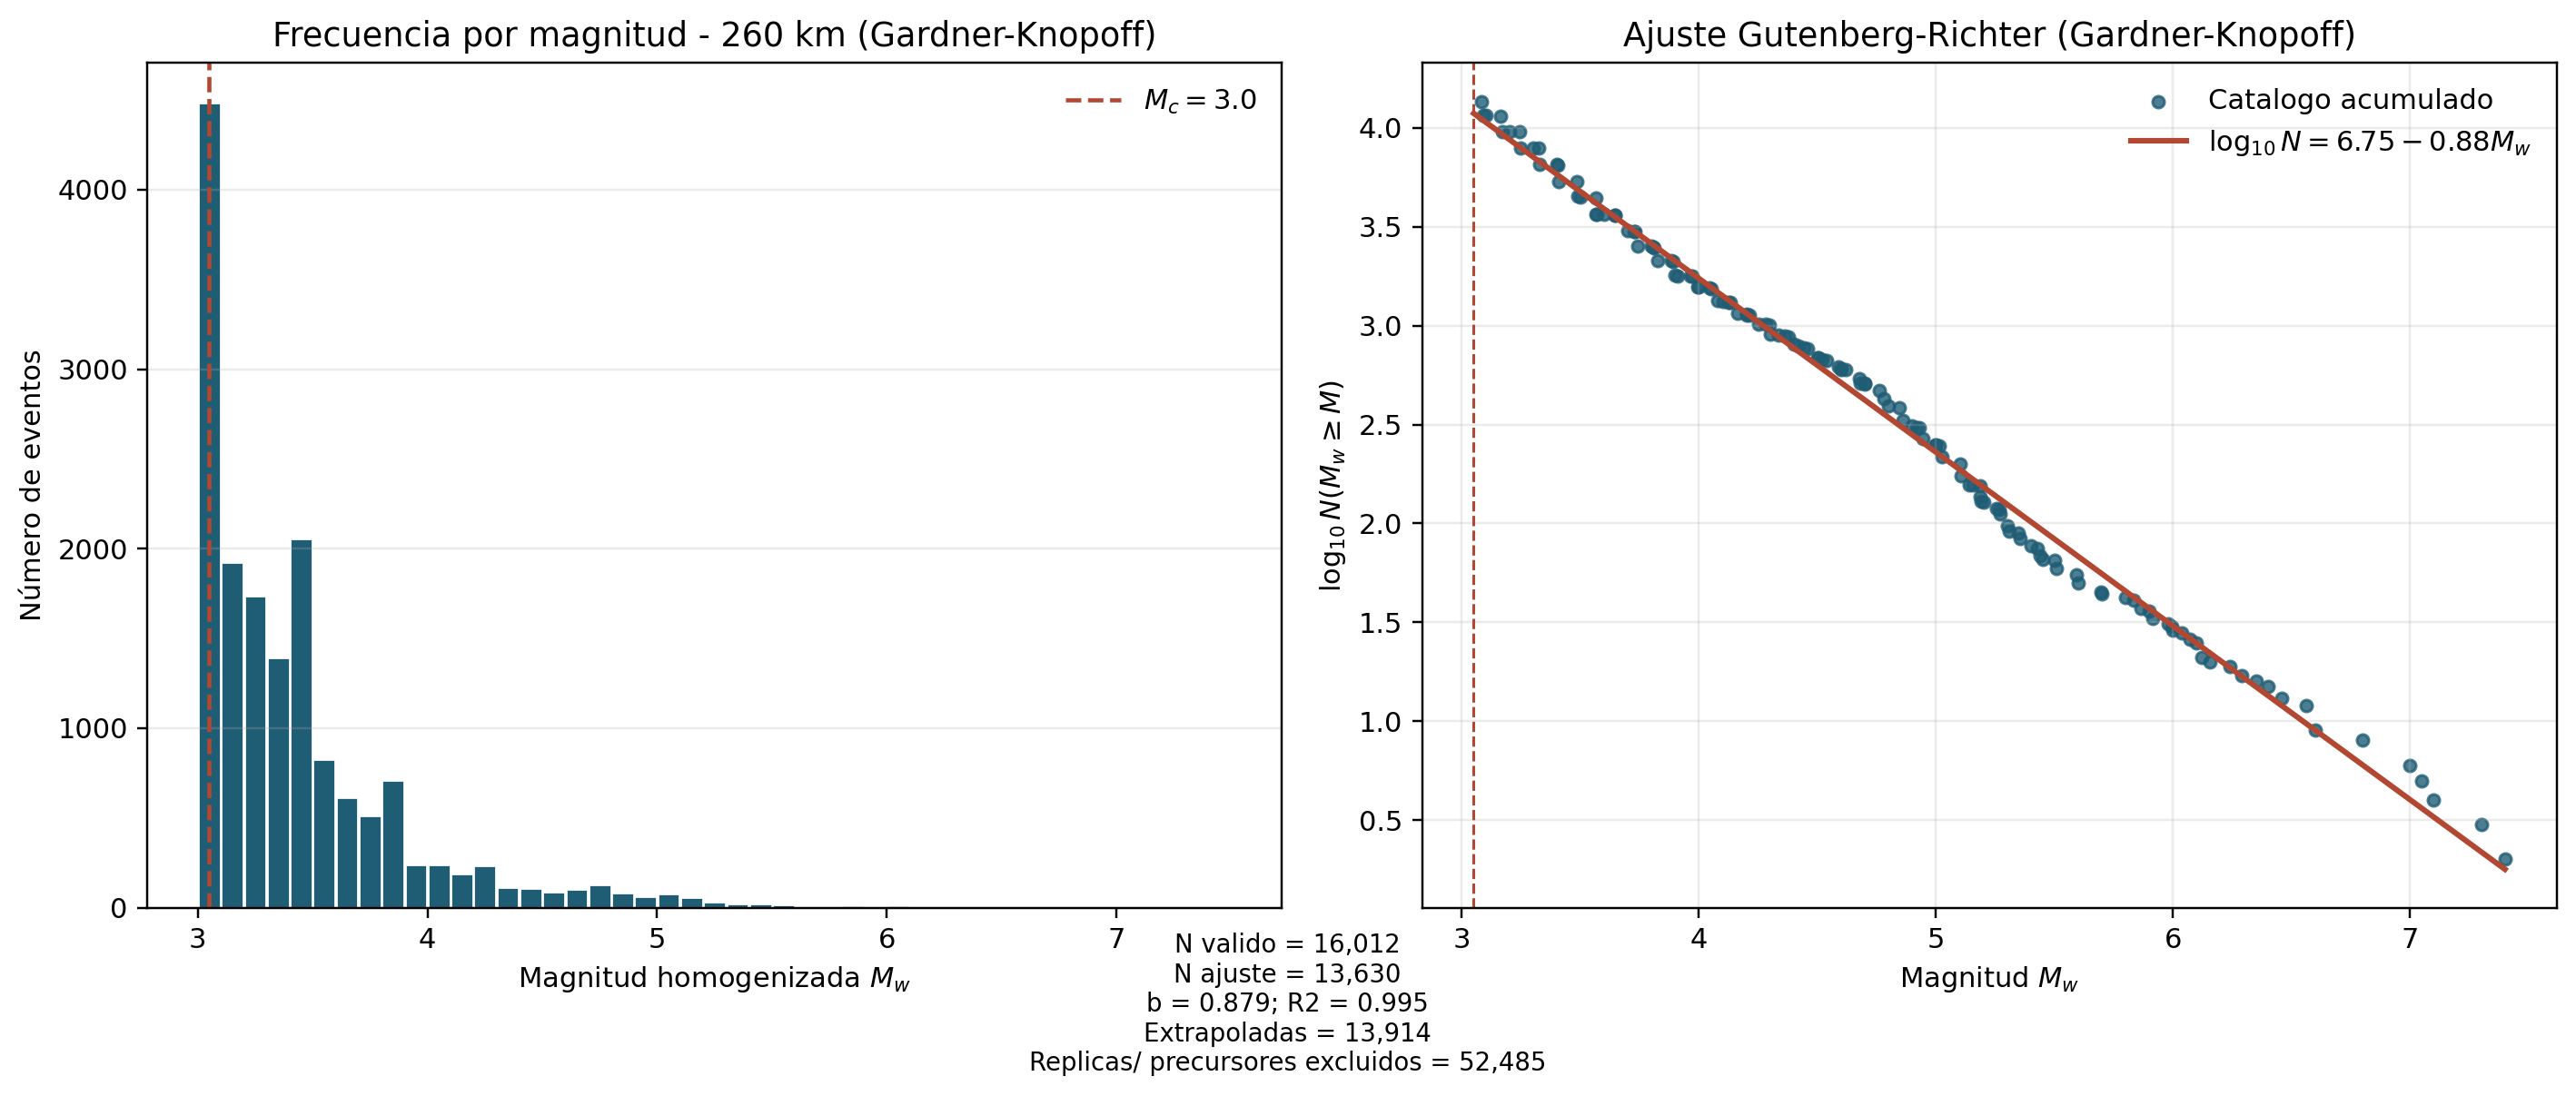
\includegraphics[width=0.92\textwidth]{../figuras/frecuencia_magnitud_260km_gk.png}
      \caption{Frecuencia y ajuste Gutenberg--Richter para el catálogo depurado a 260 km con el método Gardner--Knopoff. La línea vertical indica la magnitud de completitud exploratoria $M_c=3.05$.}
      \label{fig:frecuencia_260km}
\end{figure}

\subsection{Método de ventanas enlazadas (GKL/GKL-b)}
\label{sec:ventanas_enlazadas}

Como una alternativa intermedia entre las ventanas fijas por magnitud y la
representación basada en vecinos más cercanos, se implementó la variante de
ventanas enlazadas GKL/GKL-b. En este enfoque el evento candidato se compara
con el evento principal más fuerte que lo precede en tiempo y que cae dentro
de la ventana espacio--tiempo asociada a la magnitud más grande. Cuando la
secuencia cumple ambas condiciones simultáneamente, el miembro más débil se
marca como evento ligado a la secuencia principal y se excluye del catálogo de
mainshocks. Esta lógica conserva el esquema de depuración basado en ventanas,
pero permite enlazar la secuencia en cadena cuando varios eventos se
encuentran dentro del mismo dominio espacio--tiempo.

La comparación con los resultados de Gardner--Knopoff se presenta en el
Cuadro~\ref{tab:comparacion_decluster}, y la salida de frecuencia--magnitud
para cada radio se muestra en las Figuras~\ref{fig:frecuencia_50km_gkl} y
\ref{fig:frecuencia_260km_gkl}.

\begin{figure}[H]
      \centering
      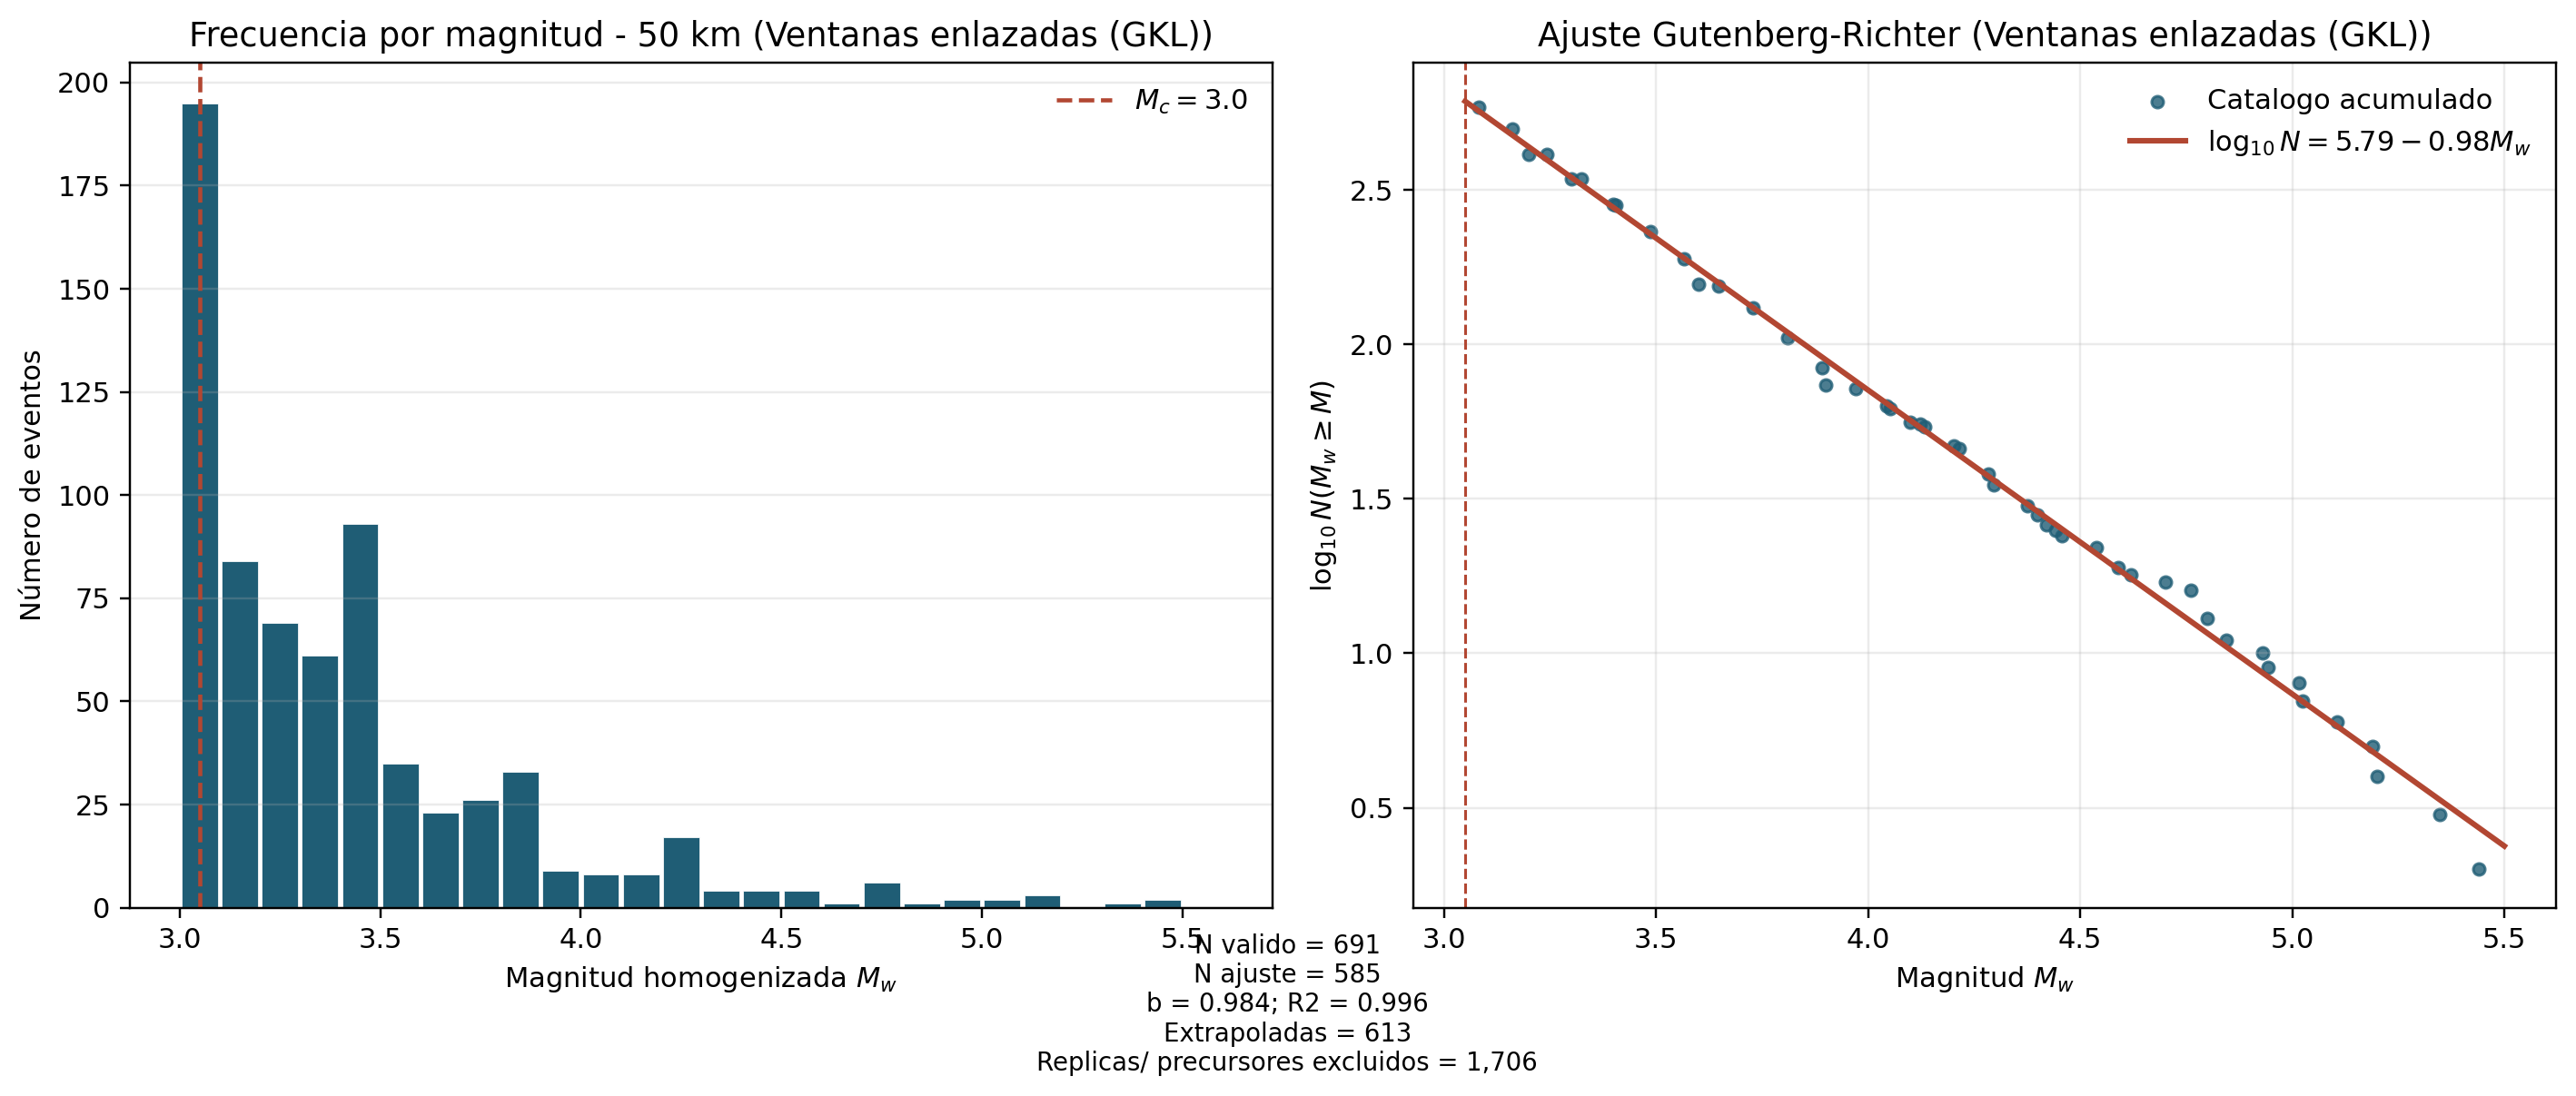
\includegraphics[width=0.92\textwidth]{../figuras/frecuencia_magnitud_50km_gkl.png}
      \caption{Frecuencia y ajuste Gutenberg--Richter para el catálogo depurado a 50 km con el método de ventanas enlazadas GKL. La línea vertical indica la magnitud de completitud exploratoria $M_c=3.05$.}
      \label{fig:frecuencia_50km_gkl}
\end{figure}

\begin{figure}[H]
      \centering
      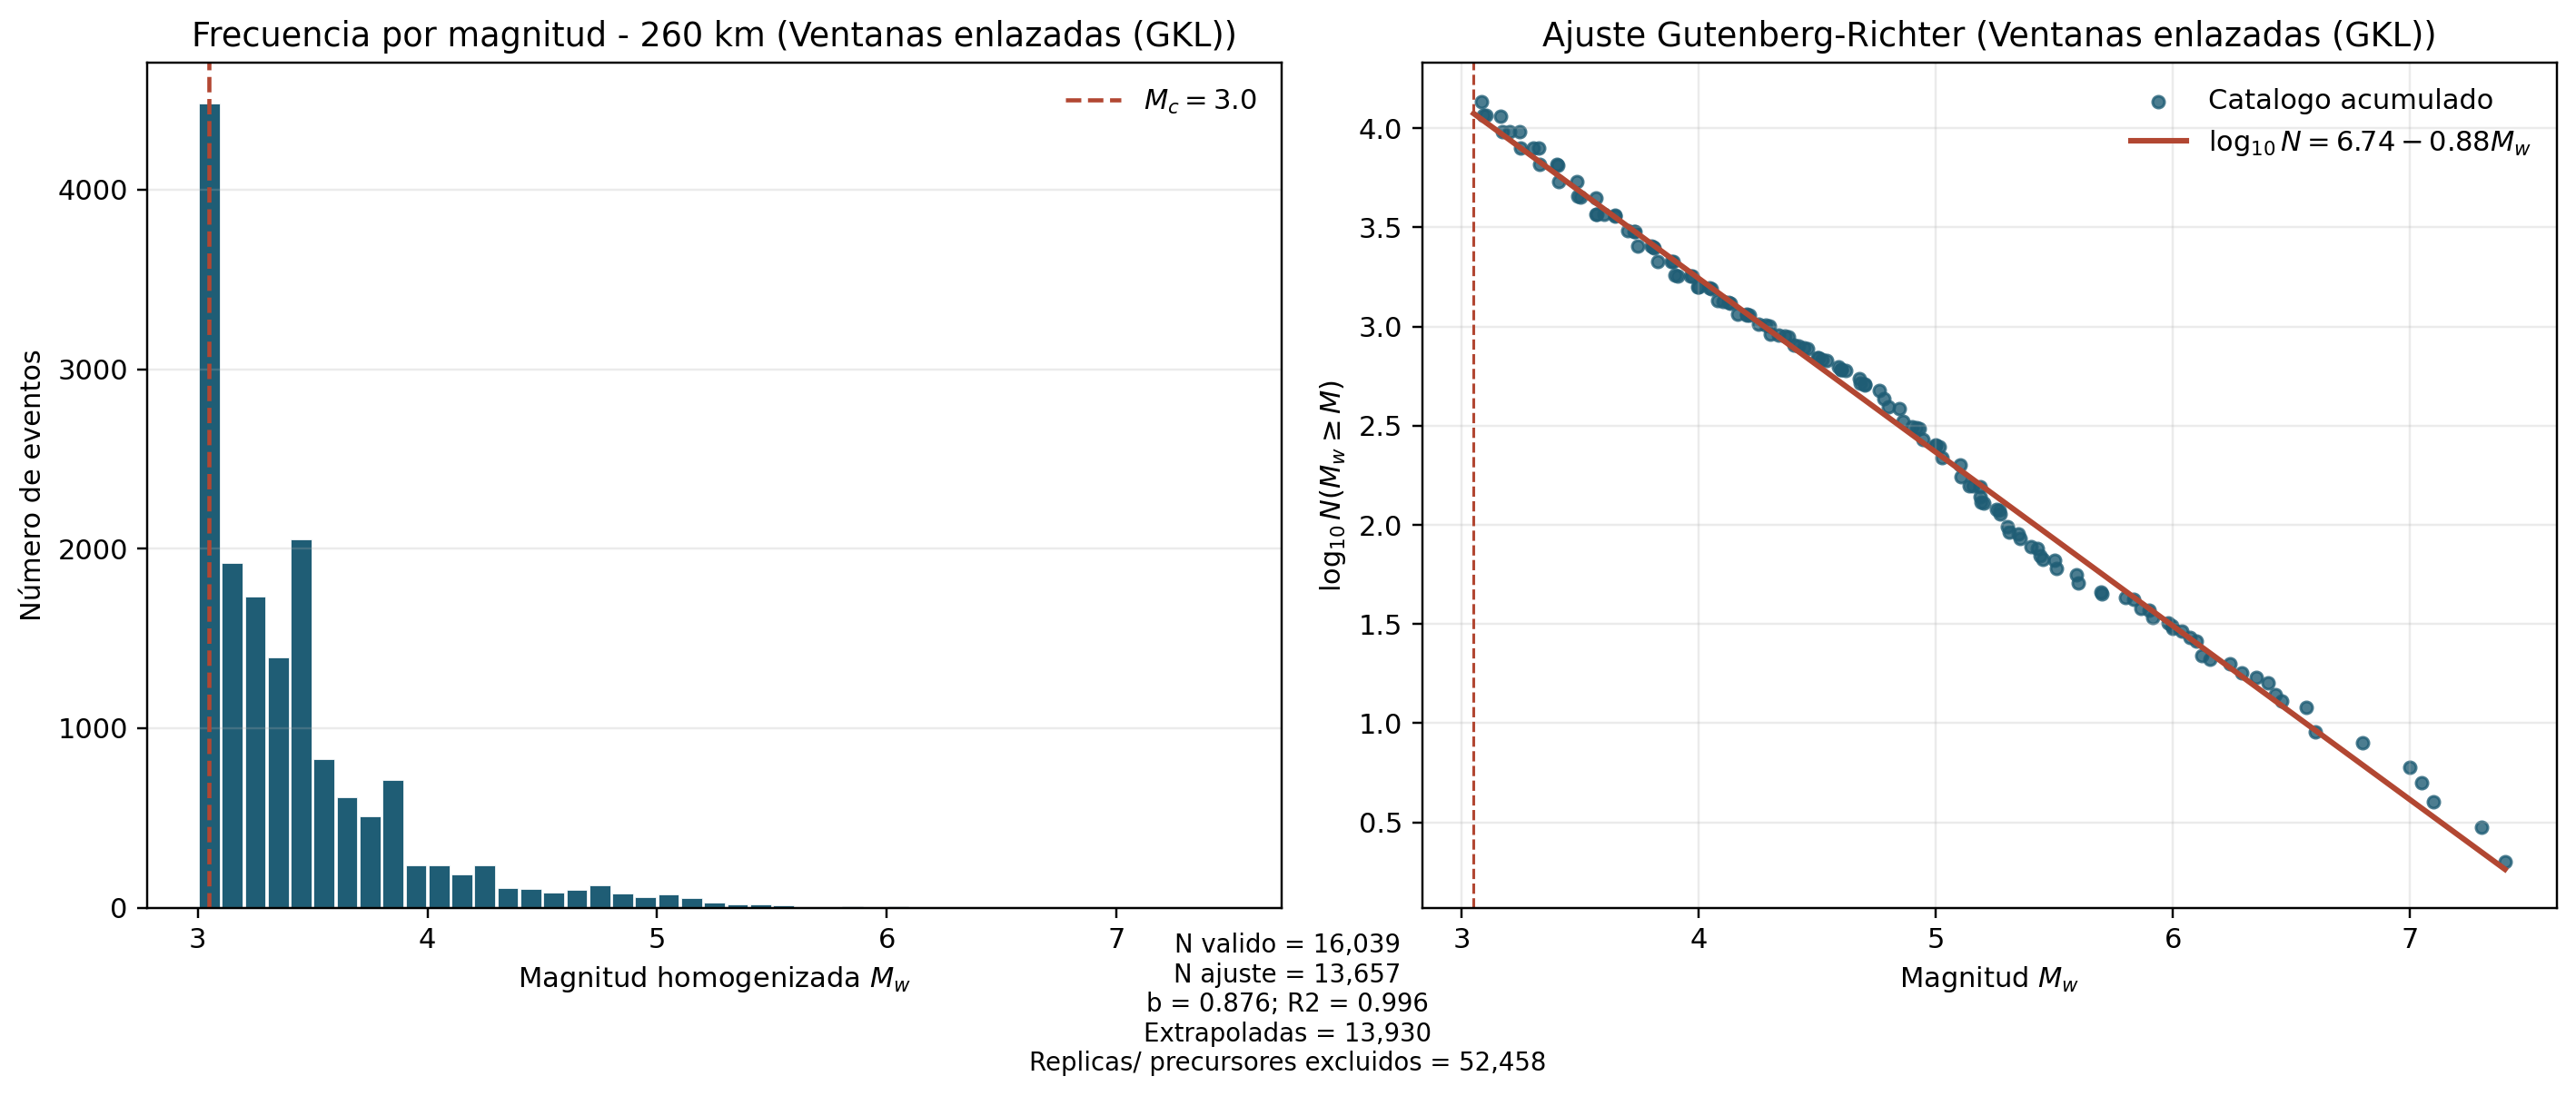
\includegraphics[width=0.92\textwidth]{../figuras/frecuencia_magnitud_260km_gkl.png}
      \caption{Frecuencia y ajuste Gutenberg--Richter para el catálogo depurado a 260 km con el método de ventanas enlazadas GKL. La línea vertical indica la magnitud de completitud exploratoria $M_c=3.05$.}
      \label{fig:frecuencia_260km_gkl}
\end{figure}

\subsection{Método de vecino más cercano (nearest-neighbor)}
\label{sec:vecino_mas_cercano}

Como comprobación de sensibilidad frente a la parametrización de la
depuración, se aplicó además el método de vecino más cercano de
Zaliapin et al. \parencite{zaliapin2008clustering} y Zaliapin y Ben-Zion
\parencite{zaliapin2013global}. En este enfoque se define una métrica basada
en la relación entre el tiempo de recurrencia y la distancia espacial con el
vecino previo más cercano, reescalados por la magnitud y por la distancia
espacial. Los eventos con valores baja de esa métrica se interpretan como
miembros de la misma secuencia, y el criterio de corte se fija sobre la
columna de la distribución empírica de la métrica.

En la práctica, se calculó la métrica de vecino más cercano para cada evento
con respecto a su predecesor temporal más cercano y se marcó como una
réplica la observación cuya métrica quedaba por debajo de un umbral de corte
asociado al percentil bajo de la distribución. Este proceso es análogo a la
lógica de declustering basada en clusters, pero utiliza una representación
rescalada en espacio--tiempo en vez de ventanas fijas por magnitud. Los
resultados obtenidos se comparan con los del método de Gardner--Knopoff en el
Cuadro~\ref{tab:comparacion_decluster}.

\begin{table}[H]
      \centering
      \caption{Comparación de depuración sobre el catálogo común $M_w>3.0$.}
      \label{tab:comparacion_decluster}
      \small
      \begin{tabular}{llrrr}
            \toprule
            Radio & Método & N. entrada & N. conservado & Eventos excluidos \\
            \midrule
            50 km  & Gardner--Knopoff & 692 & 691 & 1 \\
            50 km  & Ventanas enlazadas (GKL) & 692 & 691 & 1 \\
            50 km  & Vecino más cercano & 692 & 690 & 2 \\
            50 km  & Criterio propio & 692 & 692 & 0 \\
            260 km & Gardner--Knopoff & 16\,160 & 16\,012 & 148 \\
            260 km & Ventanas enlazadas (GKL) & 16\,160 & 16\,039 & 121 \\
            260 km & Vecino más cercano & 16\,160 & 16\,079 & 81 \\
            260 km & Criterio propio & 16\,160 & 16\,132 & 28 \\
            \bottomrule
      \end{tabular}
\end{table}

La diferencia entre ambos enfoques refleja la naturaleza distinta de los
criterios: Gardner--Knopoff usa ventanas fijas por magnitud y es más
conservador en secuencias activas del catálogo regional, mientras que el
método de vecino más cercano identifica el clúster en el espacio
rescalado tiempo--distancia, con una estrategia más dependiente de la
estructura local de cercanía en el catálogo. Para la etapa de análisis
frecuencia--magnitud, ambos métodos se aplicaron sobre el mismo catálogo
homogeneizado y se compararon con el ajuste Gutenberg--Richter.

\begin{figure}[H]
      \centering
      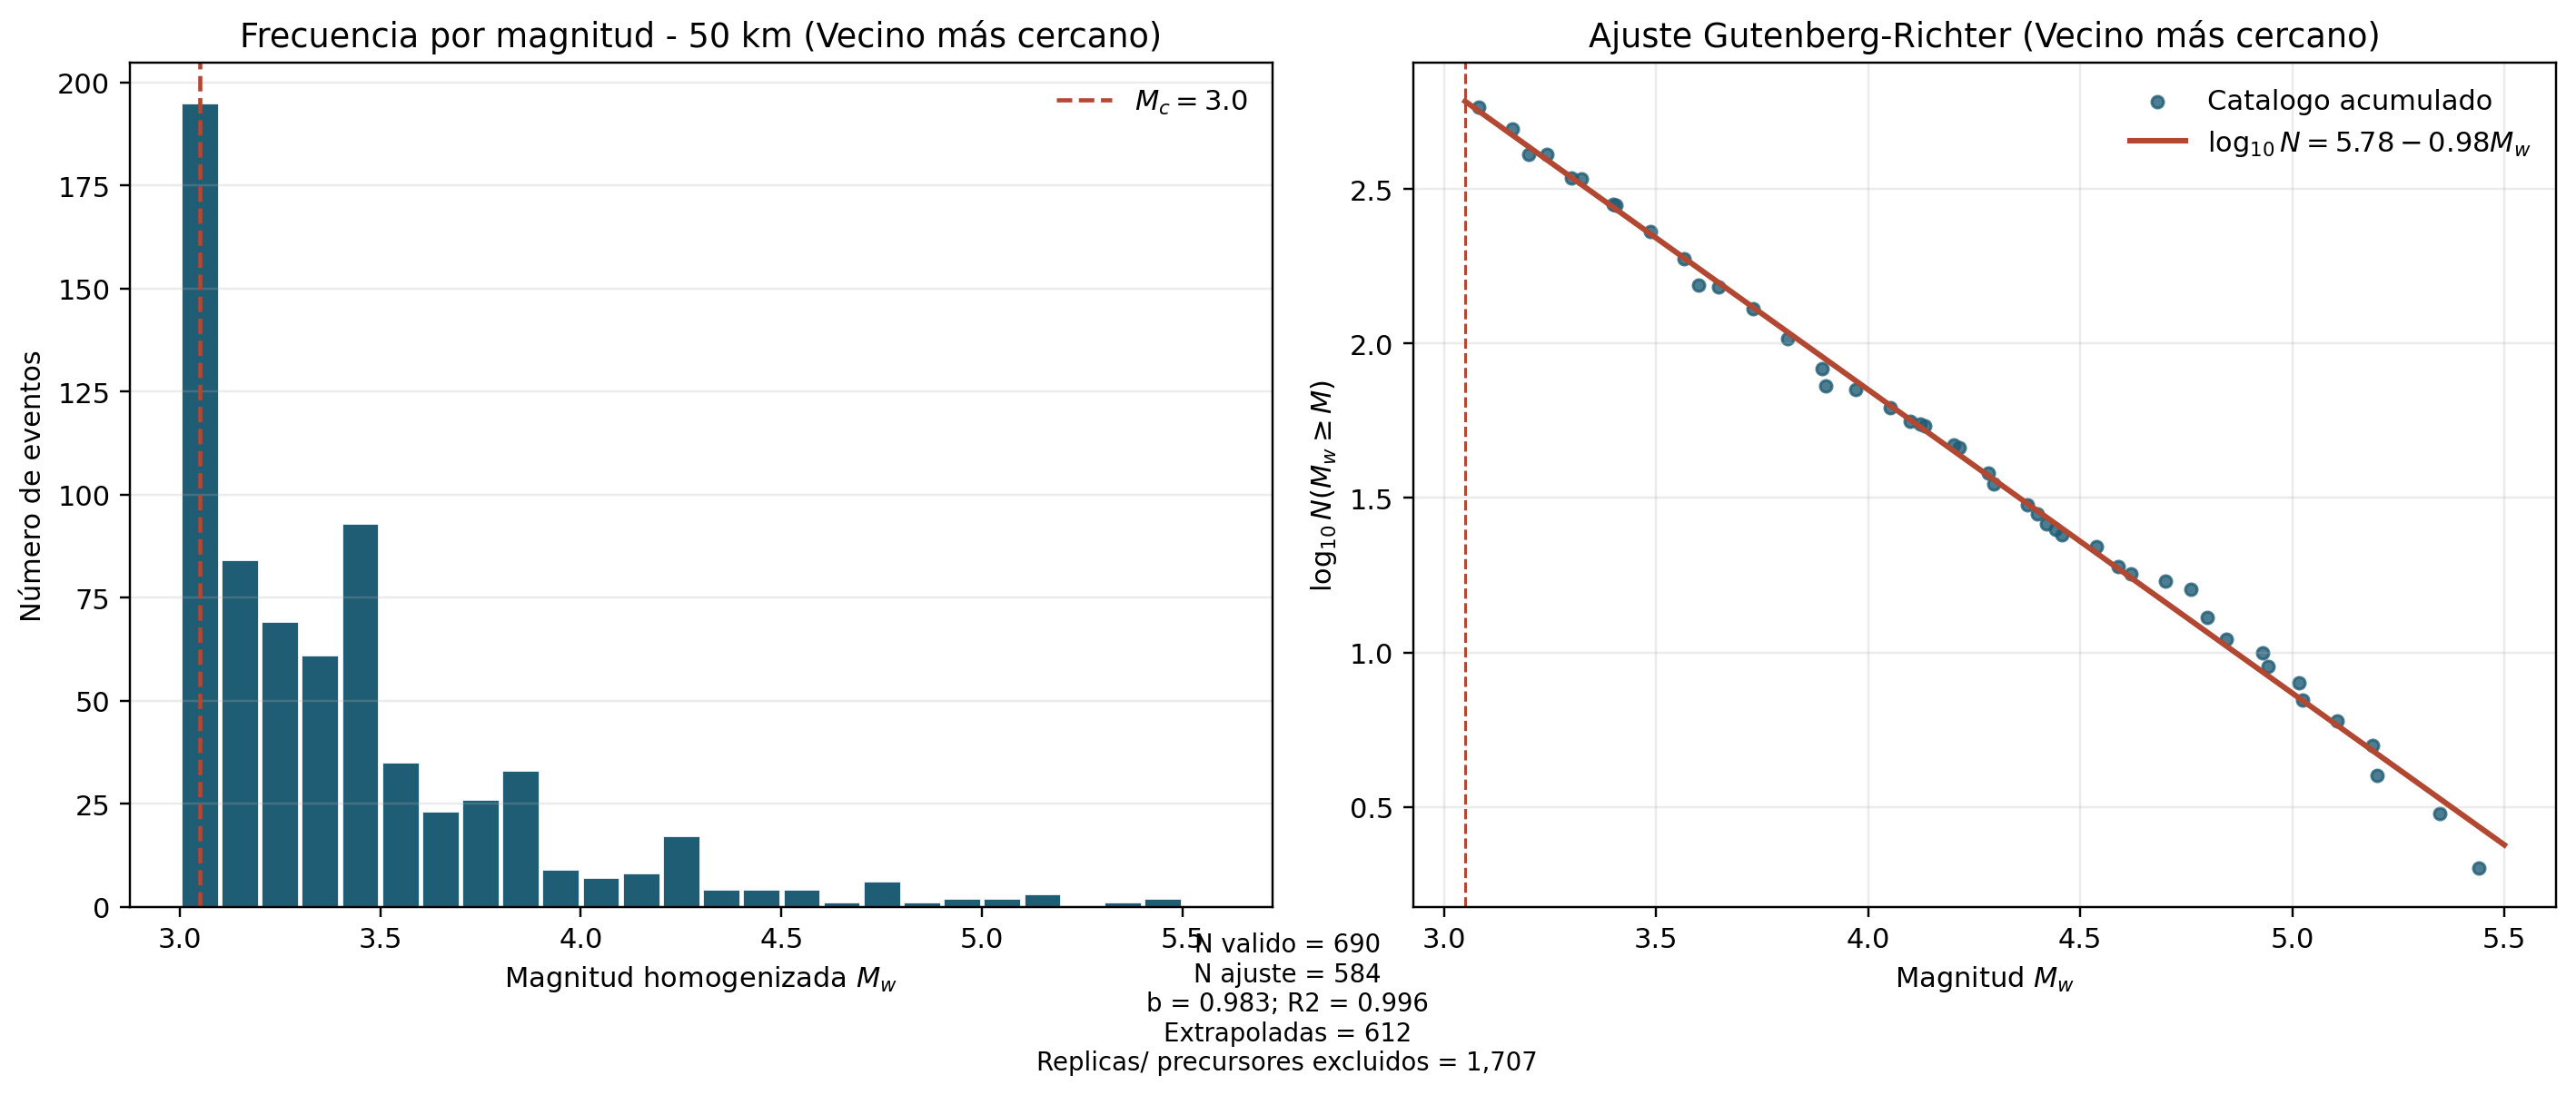
\includegraphics[width=0.92\textwidth]{../figuras/frecuencia_magnitud_50km_nn.png}
      \caption{Frecuencia y ajuste Gutenberg--Richter para el catálogo depurado a 50 km con el método de vecino más cercano. La línea vertical indica la magnitud de completitud exploratoria $M_c=3.05$.}
      \label{fig:frecuencia_50km_nn}
\end{figure}

\begin{figure}[H]
      \centering
      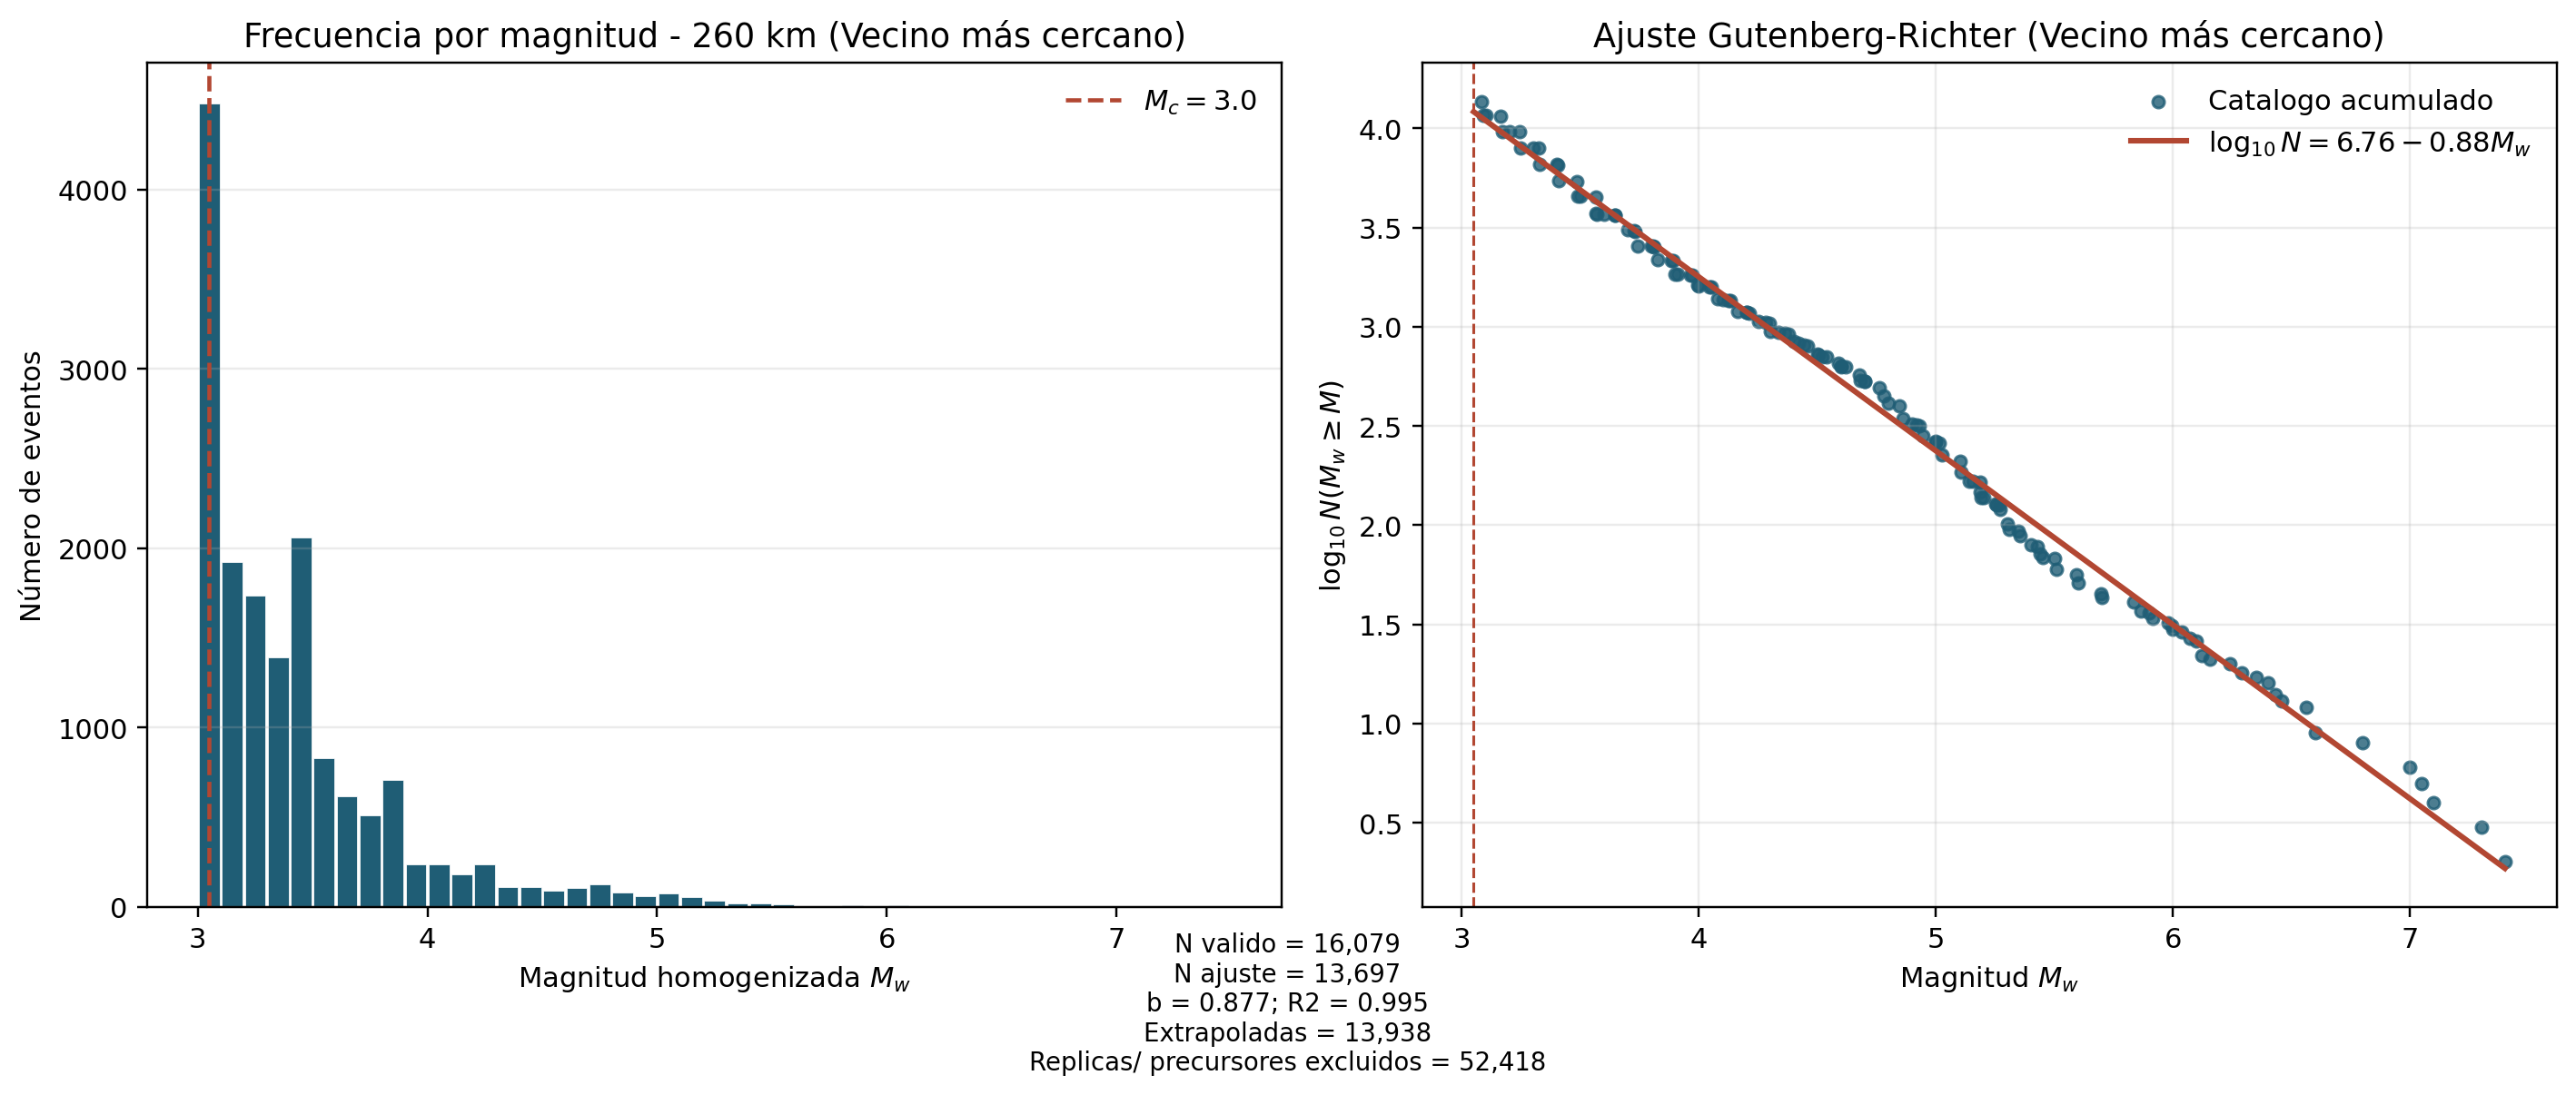
\includegraphics[width=0.92\textwidth]{../figuras/frecuencia_magnitud_260km_nn.png}
      \caption{Frecuencia y ajuste Gutenberg--Richter para el catálogo depurado a 260 km con el método de vecino más cercano. La línea vertical indica la magnitud de completitud exploratoria $M_c=3.05$.}
      \label{fig:frecuencia_260km_nn}
\end{figure}

\subsection{Criterio propio de depuración}
\label{sec:depuracion_propio}

Para establecer una alternativa independiente y comparable con los demás
métodos, este criterio se aplica únicamente
sobre el catálogo común $M_w>3.0$. Un evento se clasifica como réplica si
ocurre el mismo día, está a no más de 24 horas del principal, se encuentra a
una distancia de hasta 10 km y tiene menor magnitud que el evento principal.
En cada grupo diario se procesa primero el evento de mayor $M_w$.

El radio de 10 km es una decisión operativa del presente estudio, porque el
documento no cuantifica la expresión ``cercanos entre sí''. Este criterio no
debe confundirse con la ventana dependiente de magnitud de Gardner--Knopoff ni
con la métrica continua de vecino más cercano. La distancia se calculó
mediante la fórmula de Haversine y el archivo de salida conserva la
clasificación, el motivo de exclusión, el evento principal asociado y la
distancia calculada.

Con este criterio se conservaron 692 registros en 50 km y 16\,132 en 260 km;
los registros sin valor utilizable de $M_w$ se mantienen para trazabilidad. En
260 km se identificaron 28 réplicas por la regla espacio--temporal. Las
exclusiones por $M_w\leq3.0$ se reportan por separado en el criterio común y
no se vuelven a atribuir a este método.

\begin{figure}[H]
      \centering
      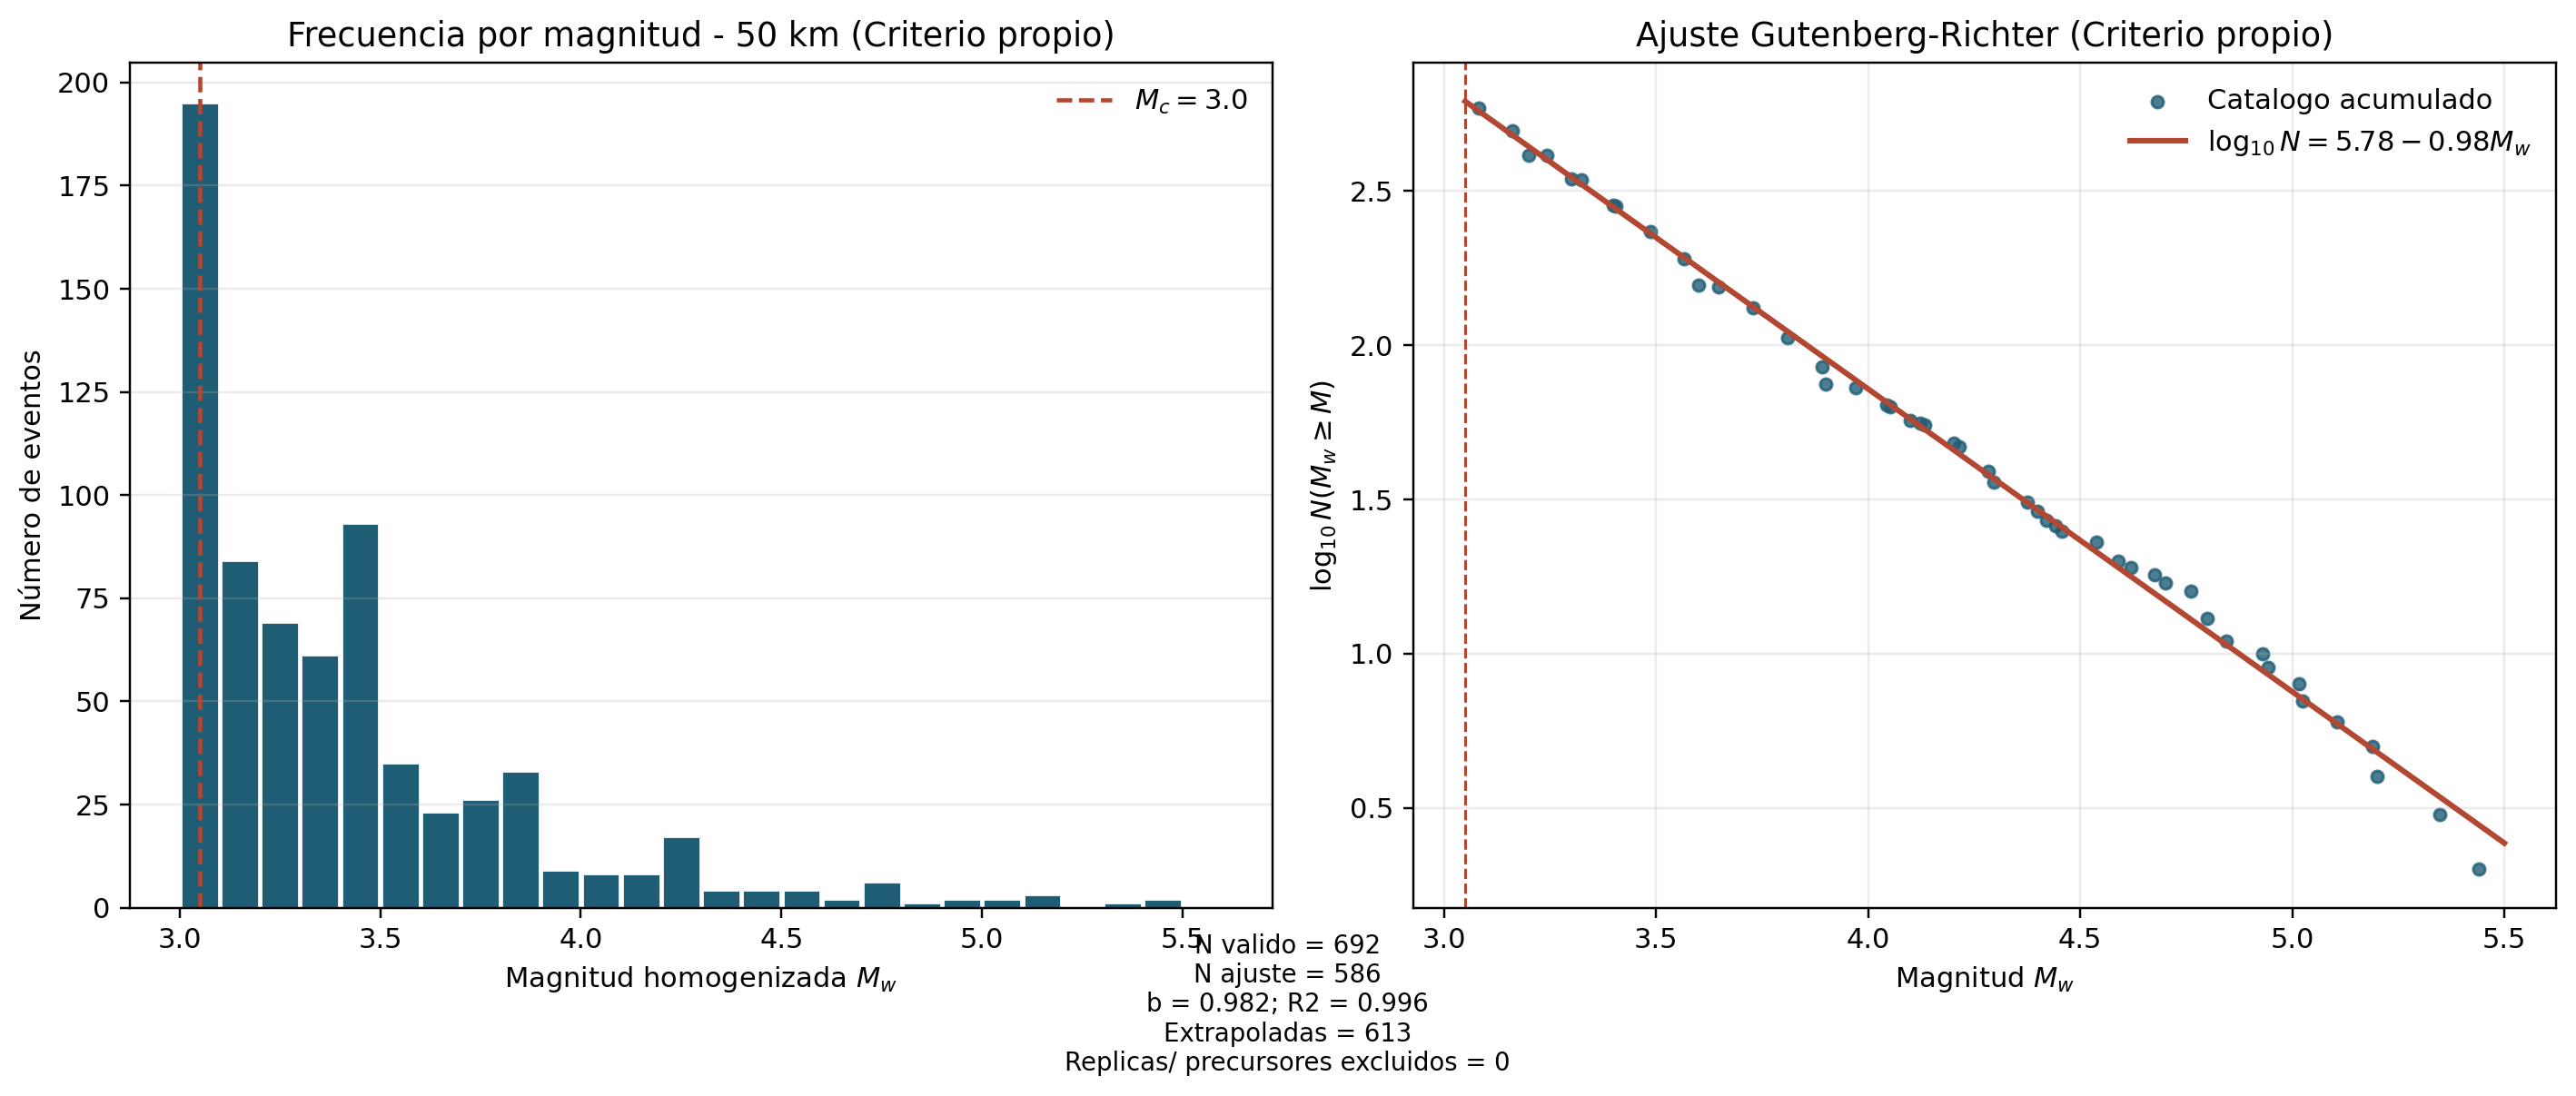
\includegraphics[width=0.92\textwidth]{../figuras/frecuencia_magnitud_50km_propio.png}
      \caption{Frecuencia y ajuste Gutenberg--Richter para el catálogo depurado a 50 km con el Criterio propio.}
      \label{fig:frecuencia_50km_propio}
\end{figure}

\begin{figure}[H]
      \centering
      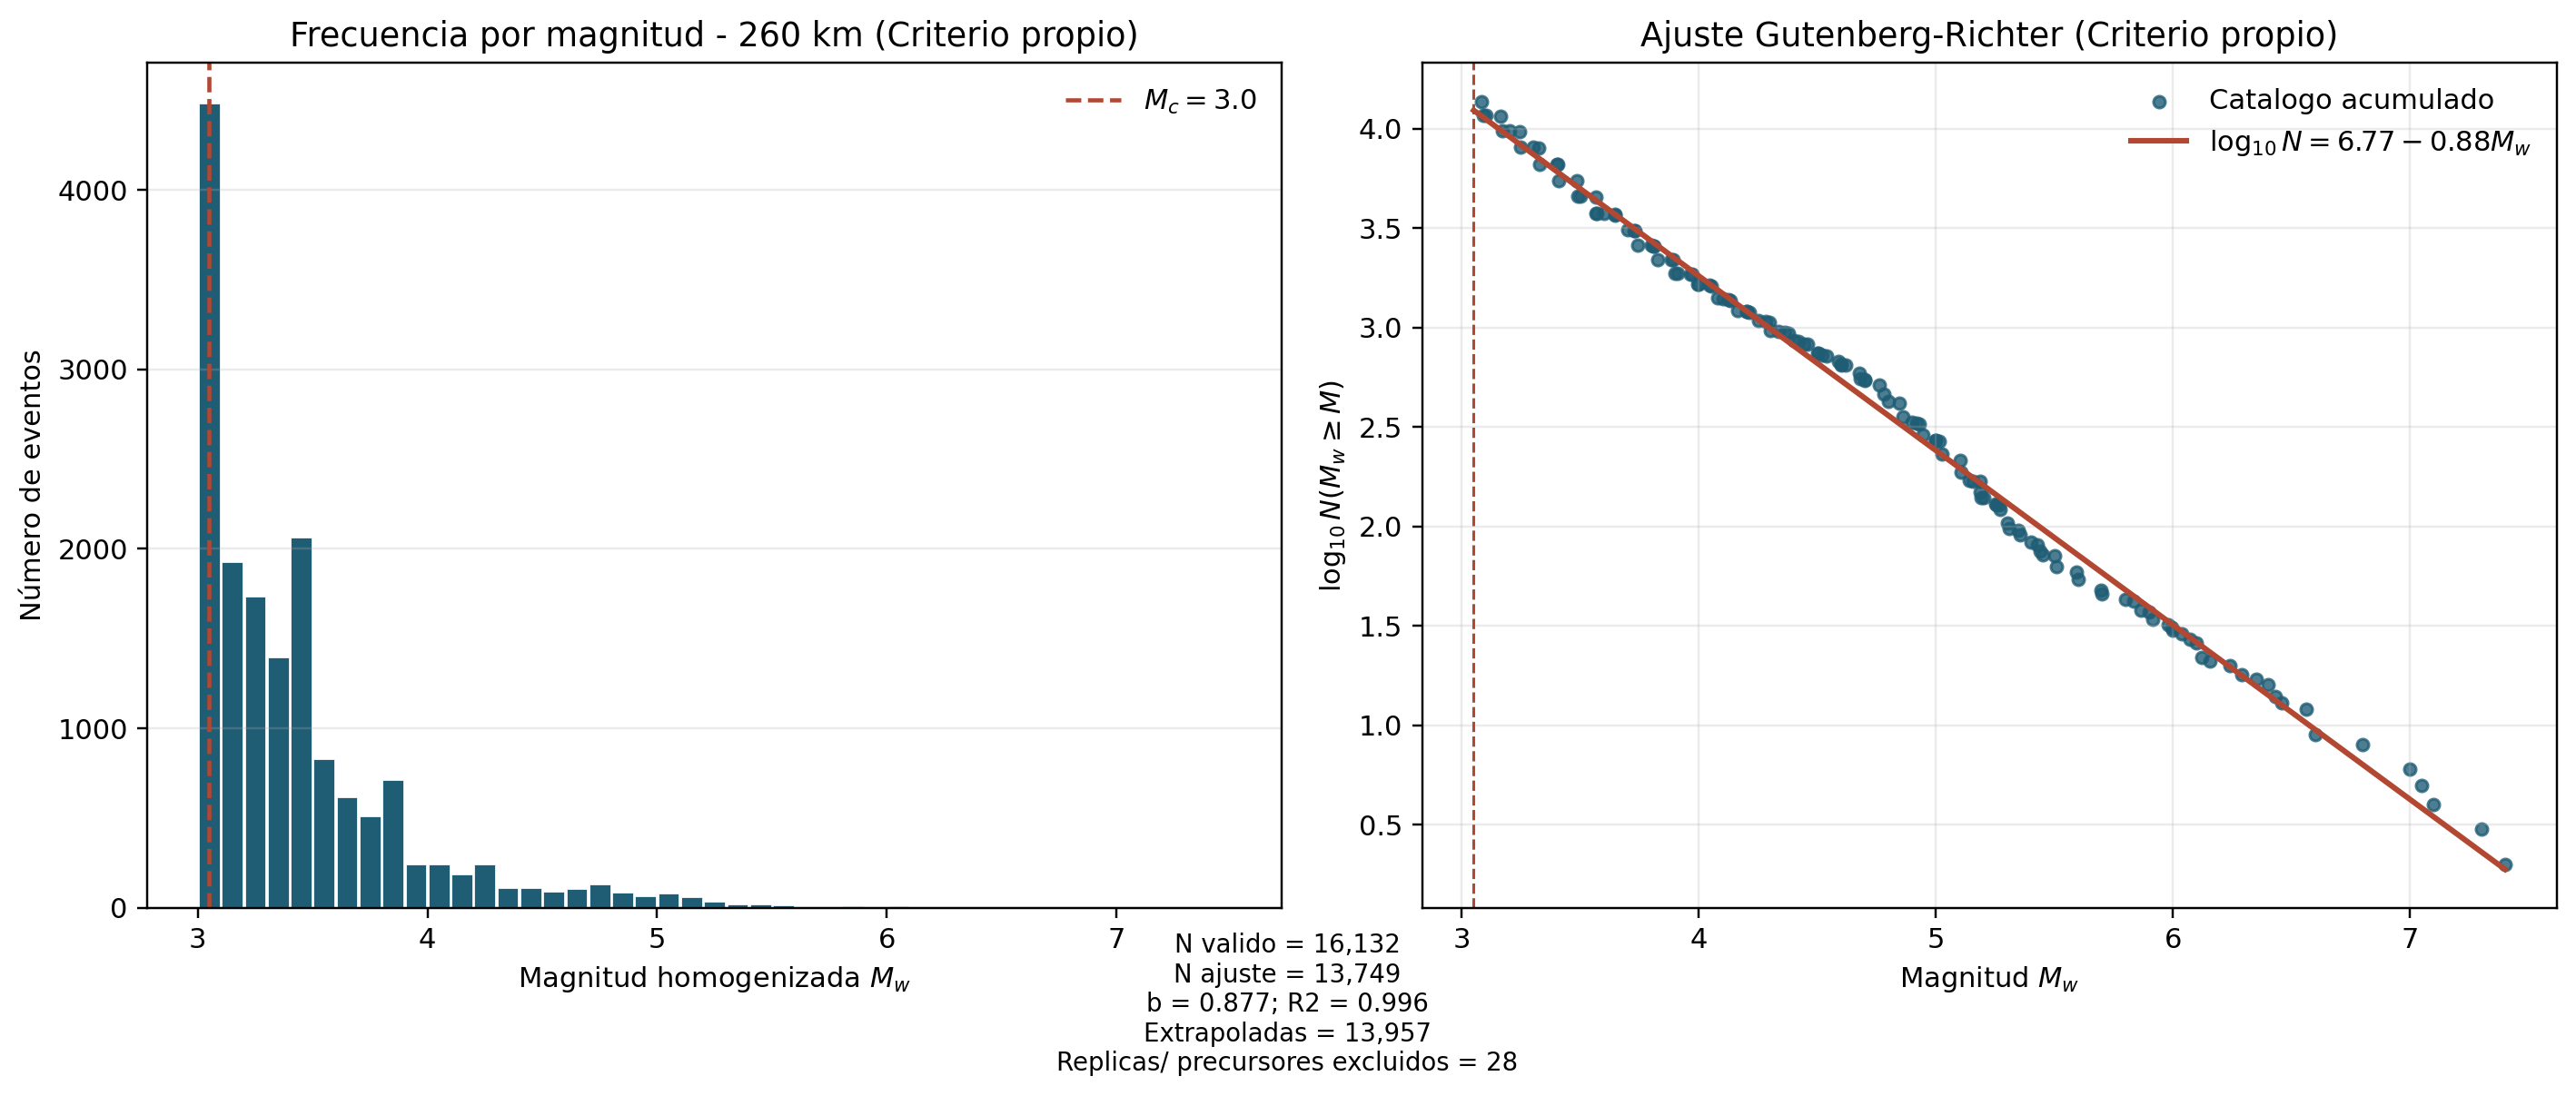
\includegraphics[width=0.92\textwidth]{../figuras/frecuencia_magnitud_260km_propio.png}
      \caption{Frecuencia y ajuste Gutenberg--Richter para el catálogo depurado a 260 km con el Criterio propio.}
      \label{fig:frecuencia_260km_propio}
\end{figure}

\subsection{Distribución frecuencia--magnitud}
\label{sec:frecuencia_magnitud}

La distribución de las magnitudes homogenizadas no se modela mediante una
distribución normal. Para la sismicidad, el modelo de referencia es la ley de
Gutenberg--Richter:
\begin{equation}
      \log_{10}N(M_w\geq M)=a-bM,
      \label{eq:gutenberg_richter}
\end{equation}
donde $N(M_w\geq M)$ es el número acumulado de eventos con magnitud igual o
mayor que $M$, $a$ representa la productividad del catálogo y $b$ controla la
proporción entre eventos pequeños y grandes. El parámetro $b$ se estima solo
por encima de la magnitud de completitud $M_c$, porque por debajo de ella la
red no necesariamente registra todos los eventos.

Para cada radio se construyó un histograma con intervalos de $0.1$ unidades de
magnitud. Se tomó como estimación exploratoria de $M_c$ el centro del intervalo
con mayor frecuencia y se ajustó una regresión lineal de
$\log_{10}N(M_w\geq M)$ contra $M_w$ para $M_w\geq M_c$. Los parámetros
obtenidos se presentan en la Tabla~\ref{tab:ajuste_gr}.

\begin{table}[H]
      \centering
      \caption{Ajuste exploratorio de Gutenberg--Richter para los catálogos depurados con los cuatro métodos.}
      \label{tab:ajuste_gr}
      \begin{tabular}{llrrrrr}
            \toprule
            Radio & Método & $N$ válido & $M_c$ & $N$ ajuste & $b$ & $R^2$ \\
            \midrule
            50 km  & Gardner--Knopoff & 691 & 3.05 & 585 & 0.984 & 0.996 \\
            50 km  & Ventanas enlazadas (GKL) & 691 & 3.05 & 585 & 0.984 & 0.996 \\
            50 km  & Vecino más cercano & 690 & 3.05 & 584 & 0.983 & 0.996 \\
            260 km & Gardner--Knopoff & 16\,012 & 3.05 & 13\,630 & 0.879 & 0.995 \\
            260 km & Ventanas enlazadas (GKL) & 16\,039 & 3.05 & 13\,657 & 0.876 & 0.996 \\
            260 km & Vecino más cercano & 16\,079 & 3.05 & 13\,697 & 0.877 & 0.995 \\
            50 km  & Criterio propio & 692 & 3.05 & 586 & 0.982 & 0.996 \\
            260 km & Criterio propio & 16\,132 & 3.05 & 13\,749 & 0.877 & 0.996 \\
            \bottomrule
      \end{tabular}
\end{table}

El ajuste es muy bueno en términos de $R^2$, pero no debe interpretarse como
prueba de que el catálogo sea físicamente homogéneo. El catálogo de 260 km
combina una red local densa del SGC, la cobertura global del USGS y un número
importante de conversiones extrapoladas; además, se observan acumulaciones en
ciertos valores de magnitud producidas por el redondeo y por las propias
correlaciones. Por ello, $b$ y $M_c$ deben recalcularse cuando se establezca la
completitud por fuente, período y tipo de magnitud, y antes de usarlos en la
estimación probabilista de amenaza.

% ============================================================
\section{Asociación de los sismos a sismofuentes}

Esta etapa queda establecida como el siguiente desarrollo del proyecto. Los
eventos depurados se asociarán espacialmente con las sismofuentes regionales,
considerando la ubicación de los epicentros, la profundidad, la geometría de
las fallas y los ambientes tectónicos relevantes para Neiva. El resultado
permitirá separar la contribución de fuentes corticales, el nido sísmico de
Bucaramanga y la subducción del Pacífico antes de construir escenarios de
amenaza.

La asociación deberá aplicar una regla geométrica reproducible, documentar los
eventos que queden sin fuente asignada y conservar la posibilidad de asignación
múltiple cuando la incertidumbre de localización o la proximidad a los límites
de una fuente lo justifique.

% ============================================================
\section{Conclusiones}

Se construyó un catálogo homogenizado a $M_w$ para radios de 50 y 260 km
alrededor de Neiva. Después del filtro común $M_w>3.0$, se aplicaron cuatro
criterios de depuración: Gardner--Knopoff, ventanas enlazadas GKL, vecino más
cercano y Criterio propio.

El Criterio propio utiliza una ventana de 24 horas, una distancia máxima de
10 km y la condición de menor magnitud frente al evento principal. Su
definición es independiente de las ventanas dependientes de magnitud y de la
métrica de vecino más cercano, por lo que sirve como comprobación adicional de
la sensibilidad del catálogo.

La magnitud de completitud $M_c=3.05$ debe interpretarse como una estimación
exploratoria derivada del centro del bin más frecuente, no como un límite físico
definitivo de la red. La siguiente fase será asociar los eventos con
sismofuentes y evaluar la completitud por fuente, período y escala de magnitud.

% ============================================================
\subsection{Trabajo futuro}

\begin{itemize}
    \item Revisar manualmente los registros \texttt{no\_convertida} y las
          magnitudes marcadas como \texttt{extrapolada}.
    \item Estimar la completitud por fuente, período y escala antes de usar
          la ley Gutenberg--Richter en amenaza sísmica.
    \item Revisar formatos de fecha, separadores decimales y profundidades
          reportadas.
    \item Revisar manualmente la sensibilidad de la depuración Gardner--Knopoff
          frente a otras tablas de ventanas y a posibles duplicados entre
          fuentes.
    \item Construcción del espectro en roca para Neiva según la NSR-10 y
          selección o generación de acelerogramas compatibles
          \parencite{nsr10}.
\end{itemize}

% ============================================================
\section*{Referencias}
\printbibliography[heading=none]

\end{document}
